\documentclass[a4paper]{report}
\usepackage{fullpage}
\usepackage{amssymb}
\usepackage{amsmath}
\usepackage{graphicx}
\usepackage{tikz}
\usepackage{tocbibind}
\usepackage{subcaption}
\usepackage{caption}
\usepackage{listings}
\usepackage{lipsum}
\usepackage{mdframed}
\usepackage{url}
\usepackage{cite}
\usepackage{dirtytalk}
\usepackage{fixltx2e}
\usetikzlibrary{calc}
\usepackage{float}
\usepackage{longtable}

\title{Business Management Processes: Verifying their Compliance with Security and Business Rules}
\author{Joanna Diep}
\begin{document}
\large
\bibliographystyle{unsrt}
\begin{titlepage}
\newcommand{\HRule}{\rule{\linewidth}{0.5mm}} % Defines a new command for the horizontal lines, change thickness here

\center % Center everything on the page

\textsc{\LARGE Imperial College London}\\[1.5cm] % Name of your university/college
\textsc{\Large Individual Project Report}\\[0.5cm] % Major heading such as course name
\textsc{\large Department of Computing}\\[0.5cm] % Minor heading such as course title

\HRule \\[0.4cm]
{ \huge \bfseries Business Management Processes: Verifying their Compliance with Security and Business Rules}\\[0.4cm] % Title of your document
\HRule \\[1.5cm]
 
\begin{minipage}{0.4\textwidth}
\begin{flushleft} \large
\emph{Author:}\\
Joanna \textsc{Diep} 
\end{flushleft}
\end{minipage}
~
\begin{minipage}{0.4\textwidth}
\begin{flushright} \large
\emph{Supervisor:} \\
Professor. Michael \textsc{Huth} \\ 
\emph{Second Marker:} \\
Dr. Anandha \textsc{Gopalan} 
\end{flushright}
\end{minipage}\\[4cm]


\includegraphics[scale=0.15]{Imperial_College_London_crest.png}\\[1cm]

{\large \today}\\[3cm] % Date, change the \today to a set date if you want to be precise
 
\vfill % Fill the rest of the page with whitespace
\end{titlepage}

\begin{abstract}
Trying to verify if a workflow is satisfiable given that there are constraints and restrictions that are placed on how and if a task can be executed is a hard problem. As businesses and companies expand and become compliant to rules and regulations, an interesting problem needs to be solved: can all the relevant tasks be executed without breaking these constraints? Otherwise if these constraints are violated, there might be a financial loss. \\

We are going to try and solve this problem using rules written in first order predicate logic to generalise the workflow and generate the relevant rules and axioms to test the satisfiability. We will then see if a set of users can be allocated to actually execute the relevant tasks. \\

We have developed an application which can handle an user input description of a workflow including its constraints. Then we must check whether the workflow is still satisfiable with the given constraints. We then finally verify what we return back is complete and correct.
\end{abstract}

\renewcommand{\abstractname}{Acknowledgements}
\begin{abstract}
I would like to whole heartedly thank my supervisor Professor. Michael Huth for his continuous and invaluable advice, feedback and support throughout the course of this project. As well as giving time for meetings to discuss ideas. \\

I would like to thank Dr. Anandha Gopalan, the second marker for their feedback and suggestions to greatly improve my report. \\

Finally, I would like to thank my family and friends for their love, support and who have had to put up with me throughout this project and throughout my time at Imperial College.  
\end{abstract}

\tableofcontents

\chapter{Introduction}
\section{Project Aims}
Over the years, enterprise systems have been growing as businesses expand. This means there is an increased need to support business processes, information flows and reporting as they become too large to manually handle. Companies are looking to make sure that their systems are protected from fraud i.e. increasing cybersecurity, and follow compliance rules and regulations that are set by governing bodies. This is because they could potentially loose a lot of money through theft or breaking the law. \\

Most companies today need to monitor these processes and keep logs of these workflows and their results to make sure that they are being compliant and that they are on record. There are many companies that already handle enterprise systems (SAP, IBM), especially cybersecurity. \\

There are many opportunities and threats within a business process if it has inconsistencies within their constraints and allocations. There are many stories in the news where businesses are constantly being attacked, where data and money can be stolen, or that businesses or individuals are fined huge sums of money for breaking compliance rules set by a particular governing or regulating body. A well known example of a compliance rule is the``Chinese Wall''\cite{ChineseWall} which is an information barrier that a business may have in order to prevent communication and exchanges of information. It may lead to a conflict of interest within an organisation, and therefore conflicts with a regulator.\\

For this reason, this project will focus on modelling these business processes, as this is very important that companies comply with rules and regulations to avoid financial penalties and risk damaging their reputation. A recent example of this is companies failing to to obey the compliance rules over social media\cite{Compliance}. Being online, it is hard to be compliant with rules from different countries without possibly breaking one. Therefore the constraints become larger and tighter within the process. \\   

There are two types of analysis that businesses use to assess: dynamic and static analysis\cite{analysis}. In this project we will be developing a tool which will implement static analysis. Static analysis is where we examine the workflow without actually executing the workflow first. However, with dynamic analysis, we would be testing and running the workflow, as they have been executed before, during run time. What is useful with this technique is that we would potentially take log files of previous workflows and do audits on them to check for compliance and to make sure there are no defects or vulnerabilities which cannot be found during static analysis. These log files can become very large; over 50GB, but they need to be kept as some checks may need to be done to test their compliance to rules and regulations. We will mainly focus on static analysis because we want to explore all the possible execution paths, not just the execution path during run time to make sure that there are no possible vulnerabilities to break the constraints. \\

The aim of the project will focus on how business processes coordinate the workflow of tasks whose execution relies on a business objective. The user should be able to input a workflow with some constraints. The application should then generate an output to say whether the workflow does not break any of the constraints and return the task executions. The user should specify these particular constraints as each workflow is different. \\

In this application, we have chosen to only cover a subset of compliance rules as there are so many and would be unrealistic to cover all the different types of rules. The description of the workflow is a command line input using a basic language. We will show how to use this language in Appendix A. 

\section{Approach}
At first, we decided that the application should be a basic language that should be able to describe a workflow along with its constraints rather than focusing on a user interface or a web application. We needed to make sure that the language would be easy to use and can efficiently express a workflow. \\

For the backend we could have implemented our own algorithm to solve these constraints over a workflow. But there are many solvers that are used for general constraint solving where the user inputs their own constraints as a theory. Constraint solvers are easy to use to validate rules and constraints subject to a workflow. We need to be able to take the input and generate the correct code for the constraint solver to be able to solve a particular workflow. A reason why we have decided not to implement our own algorithm is that these constraint solvers are generally very efficient, and some scale very well. This is what we need for this project so we can focus on some of the rules and axioms that we need to produce for each workflow. \\

There are two stages to this application: To generate the code for the constraint solver to be able to to check if the workflow satisfies all the constraints given, and to verify that these results are correct, complete and consistent with the user input. If it is not complete, there must be something wrong with either the code that was generated as passed to the constraint solver, or that there is perhaps something wrong with the constraint solver itself that it cannot solve this problem. \\

The result that we receive back from the constraint solver must be easy to read. As the workflows get larger and there are more constraints, the user must need to know what was executed in the workflow, which user was allocated to carry out the execution and under what constraints. \\

This can become a very large problem especially for businesses with a lot of compliance rules and regulations that we hit the ``P vs. NP'' problem. The larger the workflow and the more rules in place, the harder it is to test if all the rules are obeyed. We also need to be able to certify that the workflow is consistent with the result returned from the constraint solver. \\

\section{Accomplishments}
The main accomplishments that we have achieved are:
\begin{enumerate}
\item A basic language to represent a workflow as well as the user constraints which can be translated into a language readable by our constraint solver of choice.
\item Create the relevant rules and axioms for each different constraint in the workflow.
\item Return to the user whether all the constraints in the workflow has been satisfied. Also, we must return to the user the results of these constraints and what has been executed within the workflow.
\item A method to generate the corresponding code from the user input to the constraint solver language, with all the correct and corresponding rules and axioms in place. 
\item We need to verify the results returned by the constraint solver to make sure the it is correct and complete in respect to the user input. This ensures that the rules and axioms generated are the correct ones. 
\end{enumerate}

\section{Report Structure}
\begin{itemize}
\item[Chapter 2:] This section describes the background knowledge and insight into what is needed to understand this report. We will explain in more detail what workflows are and how we can express them. We will also show some main concepts of the Z3 language that we will be using throughout this report as our choice of constraint solver.  
\item[Chapter 3:] This section describes and explains some of the business rules we have implemented in this project. We also show how these can be expressed in the Z3 language. 
\item[Chapter 4:] In this section we discuss the implementation of the application. This includes creating the lexer, parser and code generator. We will also discuss how we can take the users description of a workflow using the implemented language and how we give a useful output back to the user.
\item[Chapter 5:] In the evaluation chapter, we discuss whether the constraint solver of choice is useful in real world applications and if it can scale well since theses workflows can become huge. We will also be reviewing if we have achieved all our original objectives. We will also discuss the verification of the result.
\item[Chapter 6:] Finally, the conclusion will analyse what we have actually achieved in this project as well as any interesting future work that can be accomplished on this project. 
\end{itemize}


\chapter{Background}
\section{Workflows}
\setlength{\parindent}{4em}
Business management processes can be represented as a workflow or flowchart of tasks, where each of these tasks produce a certain output for the next task to be realised. These tasks are assigned in the workflow as a sequence, where in order to perform the next task, the current task must be completed. Therefore, in order to start a task, it must meet all the constraints within workflow. However, in a large business, making sure that all the constraints are met in a workflow can become a large and hard problem as the more tasks are added to a workflow. Workflows are modeled as directed acyclic graphs\cite{AcyclicDigraph}, where there are no directed cycles. The vertices are tasks in the workflow and the directed edges connecting to each task vertex is the execution order. \\

\begin{figure}[!h]
\centering
\begin{subfigure}[b]{\textwidth}
\centering
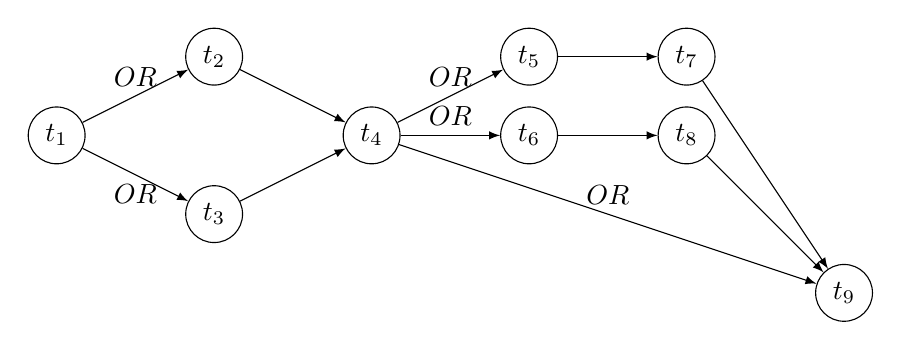
\begin{tikzpicture}
\tikzset{vertex/.style = {shape=circle,draw,minimum size=1.5em}}
\tikzset{edge/.style = {->,> = latex}} 
%\draw (0,0) circle [radius=0.5];
\node[vertex] (a) at  (0,0) {$t_{1}$};
\node[vertex] (b) at  (2,1) {$t_{2}$};
\node[vertex] (c) at (2,-1) {$t_{3}$};
\node[vertex] (d) at (4,0) {$t_{4}$};
\node[vertex] (e) at (6,1) {$t_{5}$};
\node[vertex] (f) at (6,0) {$t_{6}$};
\node[vertex] (g) at (8,1) {$t_{7}$};
\node[vertex] (h) at (8,0) {$t_{8}$};
\node[vertex] (i) at (10,-2) {$t_{9}$};
%\draw[edge] (a) to (b);
%\draw[edge] (a) to (c);
\draw[edge] (b) to (d);
\draw[edge] (c) to (d);
%\draw[edge] (d) to (e);
%\draw[edge] (d) to (f);
%\draw[edge] (d) to (i);
\draw[edge] (e) to (g);
\draw[edge] (f) to (h);
\draw[edge] (g) to (i);
\draw[edge] (h) to (i);
\path[-latex]
(a) edge node[above] {$OR$} (b)
(a) edge node[below] {$OR$} (c)
%(b) edge node[below] {} (d)
%(c) edge node[below] {} (d)
(d) edge node[above] {$OR$} (e)
(d) edge node[above] {$OR$} (f)
(d) edge node[above] {$OR$} (i);
%(e) edge node[below] {} (g)
%(f) edge node[below] {} (h)
%(g) edge node[below] {} (i)
%(h) edge node[below] {} (i);
\end{tikzpicture}
\caption{Ordered business workflow with nine tasks}
\label{fig:Business workflow with nine tasks}
\end{subfigure} \\
\begin{subfigure}[b]{\textwidth}
\centering
\begin{tabular}{ |l|l| }
\hline
Task Number & Task \\ \hline
$t_1$ & Receive order from customer \\ \hline
$t_2$ & Give total of large sale \\ \hline
$t_3$ & Give total of small sale \\ \hline
$t_4$ & Approve and authorise checkout \\ \hline
$t_5$ & Give 10\% discount \\ \hline
$t_6$ & Give 20\% discount \\ \hline
$t_7$ & Give new total of sale \\ \hline
$t_8$ & Give new total of sale \\ \hline
$t_9$ & Approve and return new total \\ 
\hline
\end{tabular}
\caption{Table of tasks}
\label{fig:Table of tasks}
\end{subfigure}
\caption{Business management process workflow}
\label{fig:Business management process workflow}
\end{figure}

An example of a business workflow is given in Figure~\ref{fig:Business workflow with nine tasks} with nine tasks that need to be allocated:
\begin{itemize}
\item A user in the business receives the order from a customer.
\item They then pass it onto another user depending on the two possible sizes of the order and are given different prices accordingly. 
\item Someone then needs to approve and authorise the price for checkout.
\item Then a discount may be provided depending on the current total cost of the order.
\item Finally, the sale is approved and the new total is returned back to the customer.
\end{itemize}

However, the order of of execution in Figure~\ref{fig:Business workflow with nine tasks} is affected by how to graph is forked. These forks are represented as constraints or rules within a business which may prevent tasks being executed such as a government restriction on business logic. The fork at task $t_{1}$ is an OR-fork showing that either task $t_{2}$ or task $t_{3}$ can be executed. Depending on whether $t_{2}$ or $t_{3}$ can be executed, determines whether task $t_{4}$ can then be executed afterwards and affects the whole execution of the workflow.  \\

\subsection{Tasks}
In business management processes, users have to be allocated tasks for an execution to occur. These tasks are represented as vertices in the graph as $t_{n}$. The tasks in the example workflow given in Figure~\ref{fig:Business workflow with nine tasks} are listed in Table~\ref{fig:Table of tasks}.\\

If users cannot be allocated to these tasks, then there is no way in which the task can be executed. Therefore it is not executed and the workflow may become unsatisfiable.\\

\subsection{Users}
A user $u$ belongs to the set of users who can be allocated to tasks in order to execute them. However, there are possible allocation constraints which refrain particular users from executing these tasks. If we have a universe of users, then we can consider two cases where $S$ is a set:

\begin{itemize}
\item Either the users in the set can be allocated in the universe of the workflow or not. In the example in Figure~\ref{fig:Set of definite users}, we can interoperate that in the set if users, Alice, Bob and Carol have been allocated, but Fred has not.
\begin{center}
$ S \triangleq f : Universe \longrightarrow \{0, 1\}$
\end{center}
\item Or that was have an extra case where we are unsure whether they can be allocated, which is represented by the $?$. Looking at Figure~\ref{fig:Set of users with unknown allocation}, we can see that Alice, Bob and Carol have been allocated in the universe of the workflow, but Fred could be allocated into the workflow. 
\begin{center}
$ S \triangleq f : Universe \longrightarrow \{0, 1, ?\}$
\end{center}
\end{itemize}

\begin{figure}[!h]
\centering
\begin{subfigure}[b]{\textwidth}
\centering
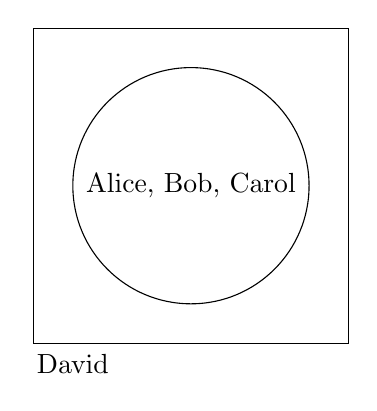
\begin{tikzpicture}
\draw (0,0) -- (4,0) -- (4,4) -- (0,4) -- cycle node[right=0.5cm, below=0.5] {David};
\draw (2,2) circle(1.5cm) node {Alice, Bob, Carol};
\end{tikzpicture}
\caption{Set of definite users}
\label{fig:Set of definite users}
\end{subfigure} \\
\begin{subfigure}[b]{\textwidth}
\centering
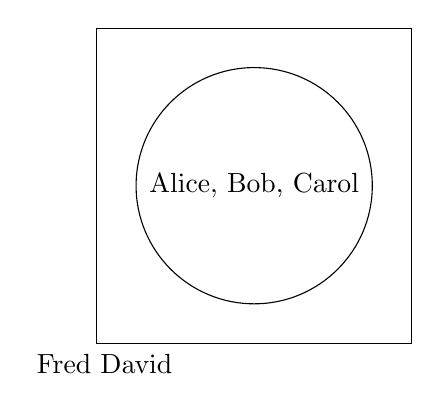
\begin{tikzpicture}
\draw (0,0) -- (4,0) -- (4,4) -- (0,4) -- cycle node[right=0.1cm, below=0.5] {Fred David};
\draw (2,2) circle(1.5cm) node {Alice, Bob, Carol};
\end{tikzpicture}
\caption{Set of users with unknown allocation}
\label{fig:Set of users with unknown allocation}
\end{subfigure}
\caption{Set of users}
\label{fig:Set of Users}
\end{figure}

\section{Business and Security Rules}
Business and security rules are used to prevent fraud and follow business compliance. For example, in some cases, different users are needed to execute a certain set of tasks to perhaps prevent fraud or erroneous activities in a workflow. In Figure~\ref{fig:Business management process workflow} some constraints about which users in the business can execute these tasks are added below:
\begin{itemize}
\item Whomever is allocated task $t_{1}$ receives the order from customers and pass them onto the relevant user. However, they cannot be allocated and execute $t_{2}$ and $t_{3}$, but can be allocated other tasks within the workflow besides $t_{2}$ and $t_{3}$.
\item Whomever is allocated task $t_{2}$ gives a total of a large sale cannot be the same user that is allocated $t_{3}$ who gives a total of a small sale. Therefore whomever is allocated $t_{3}$ cannot be allocated to $t_{2}$.
\end{itemize}

With the additional constraints to the workflow it may be satisfiable given that there are enough users. But there may be other constraints that can make this workflow unsatisfiable. For example, if there are not enough users to be allocated to ensure that some of the tasks do not have the same user. So a valid workflow is a satisfied workflow if there can be users allocated tasks in the workflow that do not break the constraints within the given model.\\

\section{Satisfiability Modulo Theories (SMT)}
Satisfiability Modulo Theories (SMT)\cite{smt_appetizer} check the satisfiability of logical formulas over given theories. It helps to determine whether there is a solution in a formula which expresses a constraint. It is one of the fundamental problems in the area of computer science to check boolean satisfiability over logical domains and the completeness and incompleteness of logical theories and complexity theory. \\

SMT is similar to Boolean or Propositional Satisfiability Problem (SAT)\cite{sat} , where the problem is to determine if there exists a determination that satisfies the boolean formula. But SAT ranges only over binary predicates which are predicates that only take in two arguments. Whereas SMT covers non-binary predicates with types and sorts. This project will focus on SMT rather than SAT as we can use non-binary predicates provided by SMT to define and solve some of these constraints. \\

\section{Z3}
Z3\cite{smt} is a SMT solver developed by Microsoft Research. It is used to integrate several decision procedures and verify the satisfiability of logical formulas over given theories. The theories our case, is the workflow model. There are many features of Z3 which will come in useful including:
\begin{itemize}
\item Uninterpreted functions - A theory that has an empty set of sentences. An example of this can be an axiom, where the satisfiability of the axiom depends on whether the uninterpreted function can be evaluated to true.
\item Linear arithmetic
\item Bitvectors, arrays, datatypes
\item Quantifiers
\item Satisfiability core
\item Returns a model
\end{itemize}

There were many other SMT solvers we considered but did not include certain built in theories and features such as:
\begin{itemize}
\item Yices\cite{yices} - It almost has all features of Z3 but doesn’t have quantifiers, which is needed to define general rules to satisfy a formula in the domain. 
\item CVC4\cite{cvc4} - It has similar features to Z3 including quantifiers, that are not included in Yices. But typically with CVC4, it is not very scalable. It is intended to run with small finite models, but realistically, business processes can be huge within large organisations.
\item MathSAT 5\cite{mathsat5}- It is lacking a lot of features in Z3, especially the quantifiers.
\end{itemize}

\subsection{Basics}
A simple example is illustrated in Figure~\ref{fig:Simple predicate logic} shows how some simple first order predicate logic in Figure~\ref{fig:Simple predicate logic using logic symbols} can be expressed in Z3 SMT solver in  Figure~\ref{fig:Simple predicate logic in Z3}.
\begin{itemize}
\item To define constants in Z3, in this case $x$ and $y$, we can declare them as constants using the keyword \texttt{(declare-const x Int)} where $x$ is the name of the constant and the type of $x$ is an Integer.
\item Z3 uses assertions to add constraints to the solver as a keyword \texttt{assert}. 
\item \texttt{(check-sat)} (line 5) is a call to Z3 to check the satisfiability of the theory. It returns \texttt{sat} if the theory is satisfiable and \texttt{unsat} if the theory is unsatisfiable.
\item \texttt{(get-model)} (line 6) is a call to Z3 to return an interpretation of the theory which makes all the formulas defined in the Z3 stack true. If the theory returns \texttt{unsat}, no model is able to be retrieved.  
\end{itemize}

In the example below, $x > 10$ is given as an assertion \texttt{(assert(> x 10))}, and $y \times 10 \geq x$ is given the assertion \texttt{(assert (>= (* y 10) x))}. When this is run in Z3, a result is returned using  \texttt{(check-sat)}. It returns as \texttt{sat} which means that this theory is satisfiable.\\ 

What we can also see, is that Z3 gives back an appropriate model as a result that satisfies these constraints with $x = 11$ and $y = 2$. This is true as if we put $x = 11$ and $y = 2$ back into the constraints, $11 > 10$ and $20 \geq 11$.
\begin{figure}[!htb]
\centering
\begin{subfigure}[b]{\textwidth}
\centering
$x > 10$ \\
$y \times 10 \geq x$
\caption{Simple predicate logic using logic symbols}
\label{fig:Simple predicate logic using logic symbols}
\end{subfigure}
\begin{subfigure}[b]{\textwidth}
\lstset{numbers=left, showspaces=false,
    showstringspaces=false, tabsize=2, breaklines=true,
    xleftmargin=5.0ex,
}
\lstset{basicstyle=\ttfamily}
\centering
\begin{lstlisting}[frame=single]
(declare-const x Int)
(declare-const y Int)
(assert (> x 10))
(assert (>= (* y 10) x))
(check-sat)
(get-model)
\end{lstlisting}
\caption{Simple predicate logic in Z3}
\label{fig:Simple predicate logic in Z3}
\end{subfigure}\\
%\end{center}
%Z3 returns a model:
%\begin{center}
\begin{subfigure}[b]{\textwidth}
\lstset{basicstyle=\ttfamily}
\begin{lstlisting}[frame=single]
sat
(model 
  (define-fun y () Int
    2)
  (define-fun x () Int
    11)
)
\end{lstlisting}
\caption{Z3 Result}
\label{fig:Z3 Result}
\end{subfigure}
\caption{Simple predicate logic}
\label{fig:Simple predicate logic}
\end{figure}

\subsection{Functions}
Z3 also has uninterpreted functions. Unlike most programming languages where functions have side effects, they may never return a value or raise or throw exceptions, Z3 functions have no side effects since they are in classical first order logic and are total.
Everything in Z3 is a function, including constants as they don’t take in arguments.
\begin{itemize}
\item \texttt{(declare-fun f (Int) Int)} - We declare a function $f$ which takes in and integer as its parameter and returns an integer
\end{itemize}

In Figure~\ref{fig:Predicate Logic with Functions}, a function \texttt{f} has been declared which takes an integer as input, and returns an integer. Since this is an uninterpreted function, Z3 does not know what this function does. But we can add some constraints, so when we apply the function to the integer, it ensures that the interpretation is consistent within the theory and constraints. \\

In Figure~\ref{fig:Z3 with functions}, there are two assertions \texttt{(assert (= (f x) x))} which represents $f(x) = x$ and \texttt{(assert (> (f y) (f x))} as $f(y) > f(x)$. The result that Z3 returns in Figure~\ref{fig:Z3 Function Result} has still kept the values of \texttt{x} and \texttt{y} as it is the same as Figure~\ref{fig:Simple predicate logic}. But for function $f$, it takes in an integer as we have specified in our function declaration as \texttt{(x!1 Int)} which means that the first variable has a type Int (integer). It returns an integer which is consistent and the type integer is interpreted. \\

Looking at the model returned in Figure~\ref{fig:Z3 Function Result}, we can see that \texttt{x} and \texttt{y} are both interpreted as a function as well as \texttt{f}. It interprets \texttt{f} to take in an integer, the \texttt{ite} stands for ``if-then-else''. So we can read the definition of \texttt{f} as ``if x!1 is equal to 20, then return 20, else if x!1 is equal to 2, then return 2 else, return 21. Else, return 20''. So for the case that \texttt{x} is put into the function \texttt{f}, then $x!1 = 20$, then the value of the function is 20, else if \texttt{y} is put into the function, then $x!1 = 2$, then the value of the function is 21. If any other input is put in, then it will return 20. \\

Z3 also includes built in arithmetic functions such as $=, -, +, \times, div, mod, \geq, \leq, >, <, not$ that support integer, real and boolean constants. \\

\begin{figure}[!htbp]
\centering
\begin{subfigure}[b]{\textwidth}
\centering
$x > 10$ \\
$y \times 10 \geq x$ \\
$f(x) = x$ \\
$f(y) > f(x)$
\caption{Predicate logic with functions}
\label{fig:Predicate logic with functions}
\end{subfigure}
\begin{subfigure}[b]{\textwidth}
\lstset{numbers=left, showspaces=false,
    showstringspaces=false, tabsize=2, breaklines=true,
    xleftmargin=5.0ex,
}
\lstset{basicstyle=\ttfamily}
\centering
\begin{lstlisting}[frame=single]
(declare-const x Int)
(declare-const y Int)
(assert (> x 10))
(assert (>= (* y 10) x))
(declare-fun f (Int) Int)
(assert (= (f x) x))
(assert (> (f y) (f x)))
(check-sat)
(get-model)
\end{lstlisting}
\caption{Z3 with functions}
\label{fig:Z3 with functions}
\end{subfigure}\\
\begin{subfigure}[b]{\textwidth}
\lstset{basicstyle=\ttfamily}
\begin{lstlisting}[frame=single]
sat
(model 
  (define-fun y () Int
    2)
  (define-fun x () Int
    20)
  (define-fun f ((x!1 Int)) Int
    (ite (= x!1 20) 20
    (ite (= x!1 2) 21
      20)))
)
\end{lstlisting}
\caption{Z3 Result with functions}
\label{fig:Z3 Function Result}
\end{subfigure}
\caption{Predicate Logic with Functions}
\label{fig:Predicate Logic with Functions}
\end{figure} 

\newpage

\subsection{Stack}
Z3 has a stack implementation, where constraints and formulas can be pushed onto and popped off the stack using the commands \texttt{(push)} and \texttt{(pop)} which pushes and pops constraints off the stack respectively. These commands can be used to check the satisfiability of some rules or definitions. When the solver stack is pushed, the state of the solver is saved. When the stack is popped, any rules and assertions declared between that pop and the corresponding push on the stack is removed from the stack, and the interpretation is reverted back to its previous state before the push.\\

In Figure~\ref{fig:Predicate Logic with stack}, the theory is satisfied before the push. However, when the stack is pushed and an assertion is added which violates the constraints already in the current frame which is $x < 2$, but $x > 2$ has been pushed onto the stack frame previously, the model becomes unsatisfied. Since the constraint $x < 2$ was between a push-pop frame, it can be popped off the stack and the model is returned back to its previous state on the stack.\\

This is useful for when we want to do some testing to see if some variables and constraints hold within a theory. We will be using these Z3 method calls for verifying the correctness and completeness of the model as well as some other tests.

\begin{figure}[H]
\centering
\begin{subfigure}[b]{\textwidth}
\lstset{numbers=left, showspaces=false,
    showstringspaces=false, tabsize=2, breaklines=true,
    xleftmargin=5.0ex,
}
\lstset{basicstyle=\ttfamily}
\centering
\begin{lstlisting}[frame=single]
(declare-const x Int)
(declare-const y Int)
(declare-fun f (Int) Int)
(assert (> x 2))
(assert (< y 2))
(assert (= (f x) (f y)))
(check-sat)
(get-model)
(push)
(assert (< x 2))
(check-sat)
(pop)
(check-sat)
(get-model)
\end{lstlisting}
\caption{Z3 with stack}
\label{fig:Z3 with stack}
\end{subfigure}\\
\begin{subfigure}[b]{\textwidth}
\lstset{basicstyle=\ttfamily}
\begin{lstlisting}[frame=single]
sat
(model 
  (define-fun y () Int
    0)
  (define-fun x () Int
    3)
  (define-fun f ((x!1 Int)) Int
    (ite (= x!1 3) 1
    (ite (= x!1 0) 1
      1)))
)
unsat
sat
(model 
  (define-fun y () Int
    0)
  (define-fun x () Int
    3)
  (define-fun f ((x!1 Int)) Int
    (ite (= x!1 3) 1
    (ite (= x!1 0) 1
      1)))
)
\end{lstlisting}
\caption{Z3 Result with stack}
\label{fig:Z3 Function stack}
\end{subfigure}
\caption{Predicate Logic with stack}
\label{fig:Predicate Logic with stack}
\end{figure} 

\newpage

\subsection{Sorts}
When a constant is defined, they are declared as a type which is a sort in Z3. For example, integers, reals and booleans are declared, they are a pre-defined sort in Z3. 
\begin{itemize}
\item \texttt{(define-sort t1 Task)} - The command defines a new symbol with the type Task.
\end{itemize}

\subsection{Quantifiers}
One of the reasons why we chose Z3 as the back end constraint solver was because it is able to have quantifiable logic such as the universal quantifier which is interpreted as \say{for all} $\forall$. The universal quantifier asserts that all predicates within the scope of the quantifier must be true of every value of the predicate. In Z3, they are represented as:
\begin{itemize}
\item \texttt{(assert (forall ((x Int)) (x > 0)))} which in first order predicate logic is $\forall x: (x > 0)$. So for all integers, they must be greater than zero.
\end{itemize}

\subsection{Satisfiability and Validity}
\subsubsection{Validity}
A formula $f$ is valid if $f$ always evaluates to true for any assignment to an appropriate value. \\

\subsubsection{Satisfiability}
A formula $f$ is satisfiable if there is some assignment to an appropriate value to the function where $f$ evaluates to true.\\

As we mentioned previously, Z3 SMT Solver gives back the satisfiability of the interpretation. It has three states when the \texttt{(check-sat)} command is called:
\begin{itemize}
\item \texttt{sat} - Satisfied model, we were able to evaluate the theory and a model can be returned. We give an example of a satisfied formula in Figure~\ref{fig:Z3 with satisfied core}.
\item \texttt{unsat} - Unsatisfied model, a model cannot be returned as the theory was not able to be evaluated. We give an example of an unsatisfied formula in Figure~\ref{fig:Z3 with unsatisfied core}.
\item \texttt{unknown} - When Z3 does not know whether a formula is satisfiable or not. Z3 cannot evaluate the theory.
\end{itemize}

What is good about whether a formula is satisfiable is that it is about finding a solution under a set of constraints. 
\begin{figure}[!htb]
\centering
\begin{subfigure}[b]{\textwidth}
\lstset{numbers=left, showspaces=false,
    showstringspaces=false, tabsize=2, breaklines=true,
    xleftmargin=5.0ex,
}
\lstset{basicstyle=\ttfamily}
\centering
\begin{lstlisting}[frame=single]
(declare-const x Int)
(assert (> x 10))
(assert (< x 100))
(check-sat)
(get-model)
\end{lstlisting}
\caption{Z3 with satisfied core}
\label{fig:Z3 with satisfied core}
\end{subfigure}\\
\begin{subfigure}[b]{\textwidth}
\lstset{numbers=left, showspaces=false,
    showstringspaces=false, tabsize=2, breaklines=true,
    xleftmargin=5.0ex,
}
\lstset{basicstyle=\ttfamily}
\begin{lstlisting}[frame=single]
(declare-const a Int)
(assert (> a 10))
(assert (< a 10))
(check-sat)
(get-model)
\end{lstlisting}
\caption{Z3 with unsatisfied core}
\label{fig:Z3 with unsatisfied core}
\end{subfigure}
\caption{Predicate Logic with stack}
\label{fig:Predicate Logic with stack}
\end{figure} 

\chapter{Theory of Business Rules}
\section{Business Management Workflows}
There are many rules and restrictions within business management workflows in order to prevent fraud, and a matter of authorisation and following regulation. Each rule is different, and therefore will have different axioms that follow. We will talk about the rules that have been implemented in the application.\\

\section{Tasks and Users}
Firstly, tasks and users need to be defined in the application in order to define the basic workflow domain. These are defined in Z3 as sorts where they define the types task and user respectively:
\lstset{showspaces=false,
    showstringspaces=false, tabsize=2, breaklines=true,
    xleftmargin=5.0ex,
}
\lstset{basicstyle=\ttfamily}
\begin{lstlisting}[frame=single]
(declare-sort Task)
(declare-sort User)
\end{lstlisting}

Then each task and user in the domain are able to be defined after the sort has been defined: 
\lstset{showspaces=false,
    showstringspaces=false, tabsize=2, breaklines=true,
    xleftmargin=5.0ex,
}
\lstset{basicstyle=\ttfamily}
\begin{lstlisting}[frame=single]
(declare-sort Task)
(declare-sort User)
(declare-const alice User)
(declare-const bob User)
(declare-const price_large_order Task)
(declare-const price_small_order Task)
\end{lstlisting}
We have now declared a user called \texttt{alice} and another user \texttt{bob} in the user domain, as well as defining two tasks in the task domain:  \texttt{receive\_large\_order} and \texttt{receive\_small\_order}. \\

\newpage

\section{User Allocation}
The most basic constraint in a workflow is that the tasks can only be executed if they have been allocated a user. Obviously, if there was not a user in the domain able to be allocated to a task, no one is able to execute and complete the task for the workflow to progress.
\begin{center}
$alloc\_user : Task \rightarrow User$
\end{center}
In Z3, we define user allocation as a function, which takes in a task, and returns a user:
\lstset{showspaces=false,
    showstringspaces=false, tabsize=2, breaklines=true,
    xleftmargin=5.0ex,
}
\begin{lstlisting}[frame=single]
(declare-fun alloc_user (Task) User)
\end{lstlisting}

Now we can allocate users to tasks. For example Alice is allocated the the checkout task:
\lstset{showspaces=false,
    showstringspaces=false, tabsize=2, breaklines=true,
    xleftmargin=5.0ex,
}
\begin{lstlisting}[frame=single]
(assert (= (alloc_user checkout) alice))
\end{lstlisting}

\section{Separation of Duty}
Separation of duties\cite{sod} is where users need to be different in order to complete a set of tasks. This is usually implemented in order to avoid conflicts of interests that may cause fraud by an individual or break some rules within a business. This restricts and reduces powers of individuals within a business where there could be a chance of collusion happening. \\

This is where a user who is allocated a task $t$, must also be a different user to who is allocated task $t\ensuremath{'}$ if these tasks are bound. This is because knowledge from task $t$ must not be used in order to execute task $t\ensuremath{'}$. It may be that separation of duties cannot use their knowledge to participate in certain tasks.\\

This is easy to spot within a workflow diagram giving in Figure~\ref{fig:Part of the example workflow}. We give a scenario that there are three users in the domain: Alice, Bob and Carol. The separation of duties are as follows: 
\begin{itemize}
\item The user who is allocated the task of receiving the order and authorising the payment at checkout and cannot not handle any form of pricing the order.
\item Whereas whichever user handles pricing of large orders cannot be the same user that handles pricing of small orders.
\end{itemize}
The same users are not authorised to be allocated the tasks of creating and authorising orders. Otherwise this could lead to the creation of fake orders or authorise orders with incorrect prices which may have the intention of benefiting themselves. It is also the case that large orders and small order prices should not be affected by each other, otherwise they could affect the final price or cause some sort of price fixing.\\

The main rules we will focus on Figure~\ref{fig:Z3 Separation of Duty} is between lines 14-18. As seen, we must give a rule that whichever user is allocated a certain task cannot be the same (not equal) as which ever user is allocated the other task which is defined in the separation of duty. 

The resulting model in Figure~\ref{fig:Z3 result for separation of duty} shows that this is in fact satisfiable under the given separation of duty constraints and the model is consistent with the description. 
\begin{center}
$alloc\_user(t) \neq alloc\_user(t\ensuremath{'})$
\end{center}
The allocation in Figure~\ref{fig:Z3 result for separation of duty} is as follows:
\begin{itemize}
\item Task price\_large\_order is allocated to user Alice.
\item Task price\_small\_order is allocated to user Bob.
\item Tasks receive\_order and checkout are both allocated to user Carol.
\end{itemize}

\begin{figure}[!h]
\begin{subfigure}{\textwidth}
\lstset{numbers=left, showspaces=false,
    showstringspaces=false, tabsize=2, breaklines=true,
    xleftmargin=5.0ex,
}
\begin{lstlisting}[frame=single]
(declare-sort Task)
(declare-sort User)

(declare-fun alloc_user (Task) User)

(declare-const alice User)
(declare-const bob User)
(declare-const carol User)
(declare-const receive_order Task)
(declare-const price_large_order Task)
(declare-const price_small_order Task)
(declare-const checkout Task)

(assert (not (= (alloc_user price_large_order) (alloc_user price_small_order))))
(assert (not (= (alloc_user price_large_order) (alloc_user checkout))))
(assert (not (= (alloc_user checkout) (alloc_user price_small_order))))
(assert (not (= (alloc_user price_large_order) (alloc_user receive_order))))
(assert (not (= (alloc_user receive_order) (alloc_user price_small_order))))

(assert (forall ((u User)) (or(= u alice)(= u bob)(= u carol))))

(check-sat)
(get-model)
\end{lstlisting}
\caption{Z3 Separation of Duty}
\label{fig:Z3 Separation of Duty}
\end{subfigure}
\end{figure}
\clearpage
\begin{figure}[!h]
\ContinuedFloat
\begin{subfigure}{\textwidth}
\lstset{numbers=none, showspaces=false,
    showstringspaces=false, tabsize=2, breaklines=true,
    xleftmargin=5.0ex,
}
\begin{lstlisting}[frame=single]
sat
(model 
  ;; universe for Task:
  ;;   Task!val!2 Task!val!3 Task!val!0 Task!val!1 
  ;; -----------
  ;; definitions for universe elements:
  (declare-fun Task!val!2 () Task)
  (declare-fun Task!val!3 () Task)
  (declare------
  ;; universe for User:
  ;;   User!val!2 User!val!0 User!val!1 
  ;; -----------
  ;; definitions for universe elements:
  (declare-fun User!val!2 () User)
  (declare-fun User!val!0 () User)
  (declare-fun User!val!1 () User)
  ;; cardinality constraint:
  (forall ((x User)) (or (= x User!val!2) (= x User!val!0) (= x User!val!1)))
  ;; -----------
  (define-fun price_small_order () Task
    Task!val!1)
  (define-fun checkout () Task
    Task!val!2)
  (define-fun receive_order () Task
    Task!val!3)
  (define-fun bob () User
    User!val!1)
  (define-fun carol () User
    User!val!2)
  (define-fun price_large_order () Task
    Task!val!0)
  (define-fun alice () User
    User!val!0)
  (define-fun alloc_user ((x!1 Task)) User
    (ite (= x!1 Task!val!0) User!val!0
    (ite (= x!1 Task!val!1) User!val!1
      User!val!2)))
)
\end{lstlisting}
\caption{Z3 result for separation of duty}
\label{fig:Z3 result for separation of duty}
\end{subfigure}
\caption{Separation of duty}
\label{fig:Separation of duty}
\end{figure}

\begin{figure}[!htb]
\centering
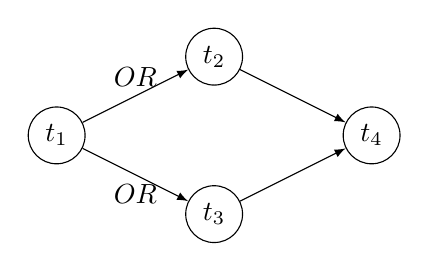
\begin{tikzpicture}
\tikzset{vertex/.style = {shape=circle,draw,minimum size=1.5em}}
\tikzset{edge/.style = {->,> = latex}} 
%\draw (0,0) circle [radius=0.5];
\node[vertex] (a) at  (0,0) {$t_{1}$};
\node[vertex] (b) at  (2,1) {$t_{2}$};
\node[vertex] (c) at (2,-1) {$t_{3}$};
\node[vertex] (d) at (4,0) {$t_{4}$};
\draw[edge] (b) to (d);
\draw[edge] (c) to (d);
\path[-latex]
(a) edge node[above] {$OR$} (b)
(a) edge node[below] {$OR$} (c);
\end{tikzpicture}
\caption{Part of the example workflow}
\label{fig:Part of the example workflow}
\end{figure}

\section{Binding of Duty}
Binding of duties\cite{bod} is where a user who is allocated a task $t$, must also be the same user who is allocated task $t\ensuremath{'}$ if these tasks are bound. This might be due to using knowledge from task $t$ to execute task $t\ensuremath{'}$. It may be that binding of duties is needed as the user who is allocated these tasks have the required knowledge in order to execute both.\\
\begin{center}
$alloc\_user(t) = alloc\_user(t\ensuremath{'})$
\end{center}

Given Figure~\ref{fig:Part of the example workflow}, who ever is allocated the task of receiving an order has to price the order, regardless of whether it is a large or small order as they may be authorised to do so. \\

As seen in Figure~\ref{fig:Z3 Binding of Duty}, the rule is specified between lines 14-17. Whichever user is allocated task price\_large\_order has to be the same (equal to) whichever user is allocated task price\_small\_order. This is matches the definition of binding of duties.\\

Looking at the result produced in Figure~\ref{fig:Z3 result for binding of duty}, this is satisfiable for the given constraints and is consistent to the user input and is complete:
\begin{itemize}
\item Task checkout is allocated to user Alice
\item All other tasks \texttt{(receive\_order, price\_large\_order, price\_small\_order)} are all allocated to user Carol. Which matches the user’s need for binding of duties.
\end{itemize}
\begin{figure}[!h]
\begin{subfigure}{\textwidth}
\lstset{numbers=left, showspaces=false,
    showstringspaces=false, tabsize=2, breaklines=true,
    xleftmargin=5.0ex,
}
\begin{lstlisting}[frame=single]
(declare-sort Task)
(declare-sort User)

(declare-fun alloc_user (Task) User)

(declare-const alice User)
(declare-const bob User)
(declare-const carol User)
(declare-const receive_order Task)
(declare-const price_large_order Task)
(declare-const price_small_order Task)
(declare-const checkout Task)

(assert (not (= (alloc_user price_large_order) (alloc_user checkout))))
(assert (not (= (alloc_user checkout) (alloc_user price_small_order))))
(assert (= (alloc_user price_large_order) (alloc_user receive_order)))
(assert (= (alloc_user receive_order) (alloc_user price_small_order)))

(assert (forall ((u User)) (or(= u alice)(= u bob)(= u carol))))

(check-sat)
(get-model)
\end{lstlisting}
\caption{Z3 Binding of Duty}
\label{fig:Z3 Binding of Duty}
\end{subfigure}
\end{figure}
\clearpage
\begin{figure}[!h]
\ContinuedFloat
\begin{subfigure}{\textwidth}
\lstset{numbers=none, showspaces=false,
    showstringspaces=false, tabsize=2, breaklines=true,
    xleftmargin=5.0ex,
}
\begin{lstlisting}[frame=single]
sat
(model 
  ;; universe for Task:
  ;;   Task!val!2 Task!val!3 Task!val!0 Task!val!1 
  ;; -----------
  ;; definitions for universe elements:
  (declare-fun Task!val!2 () Task)
  (declare-fun Task!val!3 () Task)
  (declare-fun Task!val!0 () Task)
  (declare-fun Task!val!1 () Task)
  ;; cardinality constraint:
  (forall ((x Task))
          (or (= x Task!val!2)
              (= x Task!val!3)
              (= x Task!val!0)
              (= x Task!val!1)))
  ;; -----------
  ;; universe for User:
  ;;   User!val!0 User!val!1 
  ;; -----------
  ;; definitions for universe elements:
  (declare-fun User!val!0 () User)
  (declare-fun User!val!1 () User)
  ;; cardinality constraint:
  (forall ((x User)) (or (= x User!val!0) (= x User!val!1)))
  ;; -----------
  (define-fun price_small_order () Task
    Task!val!2)
  (define-fun checkout () Task
    Task!val!1)
  (define-fun receive_order () Task
    Task!val!3)
  (define-fun carol () User
    User!val!1)
  (define-fun bob () User
    User!val!0)
  (define-fun price_large_order () Task
    Task!val!0)
  (define-fun alice () User
    User!val!0)
  (define-fun alloc_user ((x!1 Task)) User
    (ite (= x!1 Task!val!1) User!val!0
      User!val!1))
)
\end{lstlisting}
\caption{Z3 result for binding of duty}
\label{fig:Z3 result for binding of duty}
\end{subfigure}
\end{figure}

\section{Seniority}
In most businesses and corporations, there are different levels of seniority based on their positions in the company. Different seniority levels allow users to execute different tasks. For example, a confidential task maybe worked on by a less senior member of a department, but have to be authorised by a more senior member as they may have more experience or the appropriate training\cite{seniority}.\\

An example of seniority allocation is given in Figure~\ref{fig:Seniority Relationships with tasks}:
\begin{itemize}
\item Whoever is allocated $t1$ must be the same user as whoever is allocated to task $t4$ as they will have the same level of seniority, the same user will have the same seniority. From a business prospective, it does not make sense that the allocation has to have different users of the same seniority as the trust and experience levels are the same. 
\item Whoever is assigned to $t1$ has to be more senior than whoever is assigned to $t2$ and $t3$. This also means that the users assigned to $t2$ and $t3$ have to be less senior than the user allocated to $t1$.
\item The tasks $t2$ and $t3$ cannot have users of the same seniority, so therefore the users allocated to those tasks must not be the same.
\end{itemize}

We can declare a new function for seniority which takes two users as parameters and returns a boolean whether the users are senior to each other:
\begin{center}
$seniority : User \times User \rightarrow Bool$
\end{center}
\begin{lstlisting}[frame=single]
(declare-fun seniority (User User) Bool)
\end{lstlisting}

Given the example below, \texttt{u} is senior to \texttt{u\ensuremath{'}}.
\begin{lstlisting}[frame=single]
(assert (seniority (u u'))
\end{lstlisting}

The different types of seniority explained above are:
\begin{itemize}
\item $t$ has to be allocated a user that is more senior than the user allocated for $t\ensuremath{'}$ $(t > t\ensuremath{'})$: \texttt{(assert (seniority (alloc\_user t) (alloc\_user t\ensuremath{'})))}
\item $t$ has to be allocated a user that is less senior than the user allocated for $t\ensuremath{'}$ $(t < t\ensuremath{'})$: \texttt{(assert (seniority (alloc\_user t\ensuremath{'}) (alloc\_user t)))}
\item $t$ has to be allocated a user that is the same seniority as $t’$ $(t = t\ensuremath{'})$: \texttt{(assert (= (alloc\_user t) (alloc\_user t\ensuremath{'})))}
\item $t$ has to be allocated a user that is not the same seniority as $t\ensuremath{'}$ $(t != t\ensuremath{'})$: \texttt{(assert (not (= (alloc\_user t) (alloc\_user t\ensuremath{'}))))}
\end{itemize}

We give a scenario in Figure~\ref{fig:Z3 Seniority} which are expressed in lines 22-26:
\begin{itemize}
\item Whoever is allocated receive\_order has to be less senior than whoever is allocated checkout task. 
\item Also, price\_large order and price\_small\_order have to have the same seniority as each other as they are both tasks that can be executed with the same skill.
\item However, whoever is allocated receive\_order must also be less senior than the pricing tasks. 
\end{itemize}

\makeatletter
\newcommand{\srcsize}{\@setfontsize{\srcsize}{10pt}{10pt}}
\makeatother

\begin{figure}[!h]
\begin{subfigure}{\textwidth}
\lstset{numbers=left, showspaces=false,
    showstringspaces=false, tabsize=2, breaklines=true,
    xleftmargin=5.0ex,
}
\begin{lstlisting}[frame=single]
(declare-sort Task) 
(declare-sort User) 

(declare-fun seniority (User User) Bool) 

(declare-fun alloc_user (Task) User) 
(declare-fun duration (Task) Real)

(assert (forall ((u User))(not (seniority u u))))

(declare-const carol User) 
(declare-const bob User) 
(declare-const alice User) 
(declare-const checkout Task)
(declare-const price_small_order Task)
(declare-const price_large_order Task)
(declare-const receive_order Task)

(assert (seniority bob carol)) 
(assert (seniority alice bob)) 
(assert (seniority alice carol))
(assert (seniority (alloc_user checkout) (alloc_user receive_order)))
(assert (seniority (alloc_user price_small_order) (alloc_user receive_order)))
(assert (seniority (alloc_user price_large_order) (alloc_user receive_order)))
(assert (seniority (alloc_user checkout) (alloc_user receive_order)))
(assert (forall ((u User)) (or(= u carol)(= u bob)(= u alice))))

(check-sat)
(get-model)
\end{lstlisting}
\caption{Z3 Seniority}
\label{fig:Z3 Seniority}
\end{subfigure}
\end{figure}
\clearpage
\begin{figure}[H]
\ContinuedFloat
\begin{subfigure}{\textwidth}
\lstset{numbers=none, showspaces=false,
    showstringspaces=false, tabsize=2, breaklines=true,
    xleftmargin=5.0ex, basicstyle={\ttfamily\srcsize}
}
\begin{lstlisting}[frame=single]
sat
(model 
  ;; universe for User:
  ;;   User!val!2 User!val!1 User!val!0 
  ;; -----------
  ;; definitions for universe elements:
  (declare-fun User!val!2 () User)
  (declare-fun User!val!1 () User)
  (declare-fun User!val!0 () User)
  ;; cardinality constraint:
  (forall ((x User)) (or (= x User!val!2) (= x User!val!1) (= x User!val!0)))
  ;; -----------
  ;; universe for Task:
  ;;   Task!val!0 Task!val!1 Task!val!2 Task!val!3 
  ;; -----------
  ;; definitions for universe elements:
  (declare-fun Task!val!0 () Task)
  (declare-fun Task!val!1 () Task)
  (declare-fun Task!val!2 () Task)
  (declare-fun Task!val!3 () Task)
  ;; cardinality constraint:
  (forall ((x Task))
          (or (= x Task!val!0)
              (= x Task!val!1)
              (= x Task!val!2)
              (= x Task!val!3)))
  ;; -----------
  (define-fun receive_order () Task
    Task!val!1)
  (define-fun checkout () Task
    Task!val!0)
  (define-fun carol () User
    User!val!1)
  (define-fun bob () User
    User!val!0)
  (define-fun price_small_order () Task
    Task!val!2)
  (define-fun price_large_order () Task
    Task!val!3)
  (define-fun alice () User
    User!val!2)
  (define-fun seniority!16 ((x!1 User) (x!2 User)) Bool
    (ite (and (= x!1 User!val!1) (= x!2 User!val!1)) false
    (ite (and (= x!1 User!val!0) (= x!2 User!val!0)) false
    (ite (and (= x!1 User!val!2) (= x!2 User!val!2)) false
      true))))
  (define-fun k!14 ((x!1 User)) User
    (ite (= x!1 User!val!1) User!val!1
    (ite (= x!1 User!val!0) User!val!0
      User!val!2)))
  (define-fun seniority ((x!1 User) (x!2 User)) Bool
    (seniority!16 (k!14 x!1) (k!14 x!2)))
  (define-fun alloc_user ((x!1 Task)) User
    (ite (= x!1 Task!val!0) User!val!0
    (ite (= x!1 Task!val!1) User!val!1
      User!val!2)))
)
\end{lstlisting}
\caption{Z3 result for binding of duty}
\label{fig:Z3 result for binding of duty}
\end{subfigure}
\end{figure}

\begin{figure}[H]
\centering
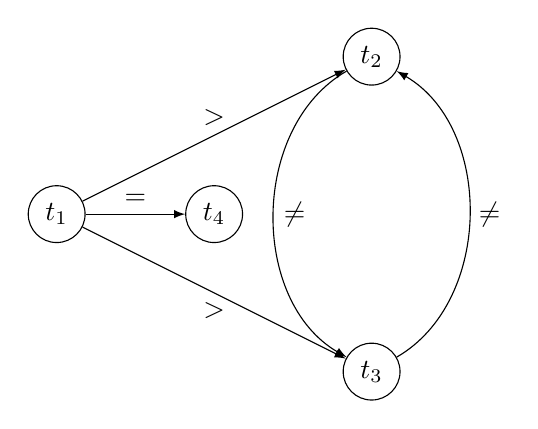
\begin{tikzpicture}
\tikzset{vertex/.style = {shape=circle,draw,minimum size=1.5em}}
\tikzset{edge/.style = {->,> = latex}} 
%\draw (0,0) circle [radius=0.5];
\node[vertex] (a) at  (0,0) {$t_{1}$};
\node[vertex] (b) at  (4,2) {$t_{2}$};
\node[vertex] (c) at (4,-2) {$t_{3}$};
\node[vertex] (d) at (2,0) {$t_{4}$};
%\draw[edge] (b)  to[bend left] (c);
%\draw[edge] (c)  to[bend left] (b);
\path[-latex]
(a) edge node[above] {$>$} (b)
(a) edge node[below] {$>$} (c)
(a) edge node[above] {$=$} (d)
(c) edge [bend right=60] node[right] {$\neq$} (b)
(b) edge [bend right=60] node[right] {$\neq$} (c);
\end{tikzpicture} \\
\begin{tabular}{ |l|l| }
\hline
Symbol & Seniority \\ \hline
$=$ & Users can be allocated this task with the same rank \\ \hline
$\neq$ & Different ranked users \\ \hline
$>$ & $t_x > t_y$ User who takes on $t_x$ is more senior than $t_y$ \\ \hline
$<$ & $t_x < t_y$ User who takes on $t_x$ is less senior than $t_y$ \\ 
\hline
\end{tabular}
\caption{Seniority Relationships with tasks}
\label{fig:Seniority Relationships with tasks}
\end{figure}

\section{Worst Time Completion}
In business, it is useful to find the worst time completion in a workflow as some task executions are not helping to optimise the total workflow duration. The aim is to then find the worst time to completion after setting rules and constraints. Users usually have finite time to execute a task and in business, there are deadline to be met. This can be established if tasks have an estimate worst time duration, the longest time it could take to execute this task. 
\begin{center}
$duration : Task \rightarrow Real$
\end{center}
We will define a function for the duration of a task and each task will have a duration listed:
\begin{itemize}
\item \texttt{(declare-fun duration (Task) Real)}
\item \texttt{(assert (= (duration t) 60))}
\end{itemize}

Task t has a worst time duration of sixty minutes to execute. Since in Z3, they do not have a time unit, the user can decide what the real value can be, i.e. minutes, hours.\\

So the worst time duration of the whole workflow would be the sum of the durations of all executed tasks.
\begin{center}
$completion\ time = \sum\nolimits_{executed(t) = true} duration(t)$
\end{center}

\newpage

\section{Temporal Order of Task Execution}
Temporal order of task execution is when tasks need to be executed in a certain order. We can easily represent this in the workflow as a directed graph, where the edges are directed to tasks (vertices) which is to be executed next. This rule is important to model in business management processes because some tasks cannot be executed before another and some tasks may be dependant on another to be executed. \\

In Figure~\ref{fig:Part of the example workflow}, it has directional arrows between vertices to represent the temporal order of task execution. For example, we cannot price orders if we have not received orders. Similarly, we cannot proceed to checkout if no pricing has been handled on the orders. We can model temporal order of task execution in Z3 where task $t$ is executed before $t\ensuremath{'}$ as:
\begin{lstlisting}[frame=single]
(declare-fun before (Task Task) Bool)
(assert (before t t'))
\end{lstlisting}

\section{Task Execution (and, or, exclusive-or)}
Another constraint we are going to explore is which tasks are actually executed. In some workflows some tasks are not necessarily needed to be executed. Given in Figure~\ref{fig:Part of the example workflow}, we can create a fork at task \texttt{receive\_order} and determine which pricing task is next to be executed. We can have three different types of forking:
\begin{itemize}
\item And - All tasks in the forking have to be executed, we cannot choose which tasks to execute.
\item Or - One or more tasks in the forking have to be executed, we cannot choose to execute none.
\item Exclusive or - One and only one task can be executed.
\end{itemize}

We can define a function \texttt{executed} to express which tasks are actually being executed. The function takes a task as a parameter and returns a boolean, whether the task has been executed or not.
\begin{center}
$executed : Task \longrightarrow Bool$
\end{center}
\begin{lstlisting}[frame=single]
(declare-fun executed (Task) Bool)
\end{lstlisting}

We assume that if the input has not explicitly stated that there is an or fork or an exclusive-or fork, that they are all and-forks. All tasks must be allocated and executed. So in the example workflow below, all tasks $t_1, t_2, t_3, t_4$ must be allocated and executed. \\

So to express all executed tasks, where all tasks are executed:
\begin{lstlisting}[frame=single]
(assert (executed t))
\end{lstlisting}
\begin{center}
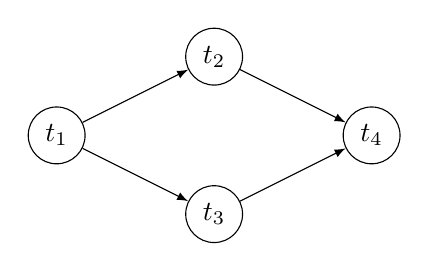
\begin{tikzpicture}
\tikzset{vertex/.style = {shape=circle,draw,minimum size=1.5em}}
\tikzset{edge/.style = {->,> = latex}} 
%\draw (0,0) circle [radius=0.5];
\node[vertex] (a) at  (0,0) {$t_{1}$};
\node[vertex] (b) at  (2,1) {$t_{2}$};
\node[vertex] (c) at (2,-1) {$t_{3}$};
\node[vertex] (d) at (4,0) {$t_{4}$};
\draw[edge] (b) to (d);
\draw[edge] (c) to (d);
\draw[edge] (a) to (b);
\draw[edge] (a) to (c);
\end{tikzpicture}
\end{center}

To express an or fork, one or more tasks can be allocated and executed. In the example bewlow, at task $t_1$ either $t_2$ or $t_3$ or both can be executed and therefore allocated:
\begin{lstlisting}[frame=single]
(assert (or (and (executed t1) (executed t2))(and (executed t1) (executed t3))))
\end{lstlisting}
\begin{figure}[!htb]
\centering
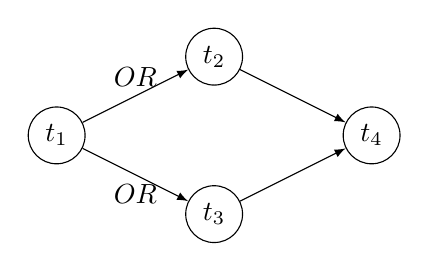
\begin{tikzpicture}[cloud/.style={
      draw=black,
      thick,
      ellipse,
      fill=red!20,
      minimum height=2em
    }]
\tikzset{vertex/.style = {shape=circle,draw,minimum size=1.5em}}
\tikzset{edge/.style = {->,> = latex}} 
%\draw (0,0) circle [radius=0.5];
\node[vertex] (a) at  (0,0) {$t_{1}$};
\node[vertex] (b) at  (2,1) {$t_{2}$};
\node[vertex] (c) at (2,-1) {$t_{3}$};
\node[vertex] (d) at (4,0) {$t_{4}$};
\draw[edge] (b) to (d);
\draw[edge] (c) to (d);
\path[-latex]
(a) edge node[above] {$OR$} (b)
(a) edge node[below] {$OR$} (c);
\end{tikzpicture}
\caption{Over constrained workflow}
\label{fig:Over constrained workflow}
\end{figure}

To express an exclusive-or fork, similar to the or fork, but only $t_2$ or $t_3$ can be executed, but not both.
\begin{lstlisting}[frame=single]
(assert (xor (and (executed t1) (executed t2))(and (executed t1) (executed t3))))
\end{lstlisting}

\begin{figure}[!h]
\centering
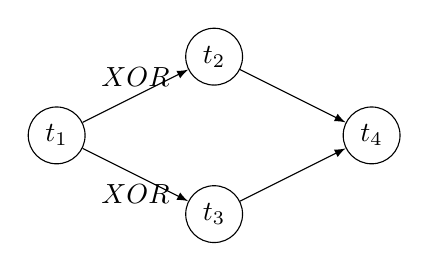
\begin{tikzpicture}
\tikzset{vertex/.style = {shape=circle,draw,minimum size=1.5em}}
\tikzset{edge/.style = {->,> = latex}} 
%\draw (0,0) circle [radius=0.5];
\node[vertex] (a) at  (0,0) {$t_{1}$};
\node[vertex] (b) at  (2,1) {$t_{2}$};
\node[vertex] (c) at (2,-1) {$t_{3}$};
\node[vertex] (d) at (4,0) {$t_{4}$};
\draw[edge] (b) to (d);
\draw[edge] (c) to (d);
\path[-latex]
(a) edge node[above] {$XOR$} (b)
(a) edge node[below] {$XOR$} (c);
\end{tikzpicture}
\caption{Over constrained workflow}
\label{fig:Over constrained workflow}
\end{figure}

\newpage

\section{Authorised User Allocation}
In a business process, we can choose the authorise particular users to execute a task explicitly. This is similar to RBAC\cite{rbac} where a system restricts access to authorised users in a domain. Authorisation is usually assigned to them by their roles. We have not implemented roles in the set of workflow constraints, but rather just users who are only allowed by input. If there are more than one users authorised to execute a task, then we can use Z3 to choose which user to execute the task. So either users Alice or Bob can be allocated the task of receiving the order to be executed and only them:
\begin{lstlisting}[frame=single]
(assert (or (=(alloc_user receive_order) alice) 
(= (alloc_user receive_order) bob)))
\end{lstlisting}


\chapter{Implementation}
\section{Project Focus}
The main aim of this project is to design a simple language in which constraints on execution of tasks within a workflow can be specified. The result that should be returned is whether the workflow is satisfiable or not, subject to all the constraints. Also, the model returned should be easy to read and understandable to the user. We also need to verify that the model returned to the user is complete and consistent to the user input.\\

The first discussion was whether to implement an algorithm that would solve these constraints or to use a back-end constraint solver. The benefit of using a back-end constraint solver like Z3 is that these algorithms are very efficient, perhaps more efficient than if it was implemented from scratch in this project. The application is built using the language  Python\cite{python} and the Z3 python module\cite{Z3Python} as the back-end constraint solver. \\

The language is a simple language which can be read a s a file or through command line prompt. This is where the universe of tasks and users are defined. There are also predefined tokens which define certain constraints on a workflow as well as axioms and rules, both of which the user has specified and default ones that are for more general workflows. The application interprets the workflow described in the language and checks if the workflow is satisfiable and gives back a suitable model.\\

\section{Application Outline}
The basic outline of this application is given in Figure~\ref{fig:Application outline}.
\begin{itemize}
\item Firstly, the user inputs the language as either a file containing syntax for a workflow or command line input of a workflow.
\item Then the application, which is written in Python interoperates the input.
\item The lexer tokenises the input and the parser parses the input.
\item After parsing, the Z3 SMT code is generated.
\item The result is handled to check whether the workflow is satisfiable given the constraints.
\item The resulting model is verified and certified to make sure that the resulting model is consistent with the user input.
\item Depending on whether the workflow was satisfiable and whether it was verified determines if a model will be returned to the user.
\end{itemize}

\begin{figure}[!h]
\centering
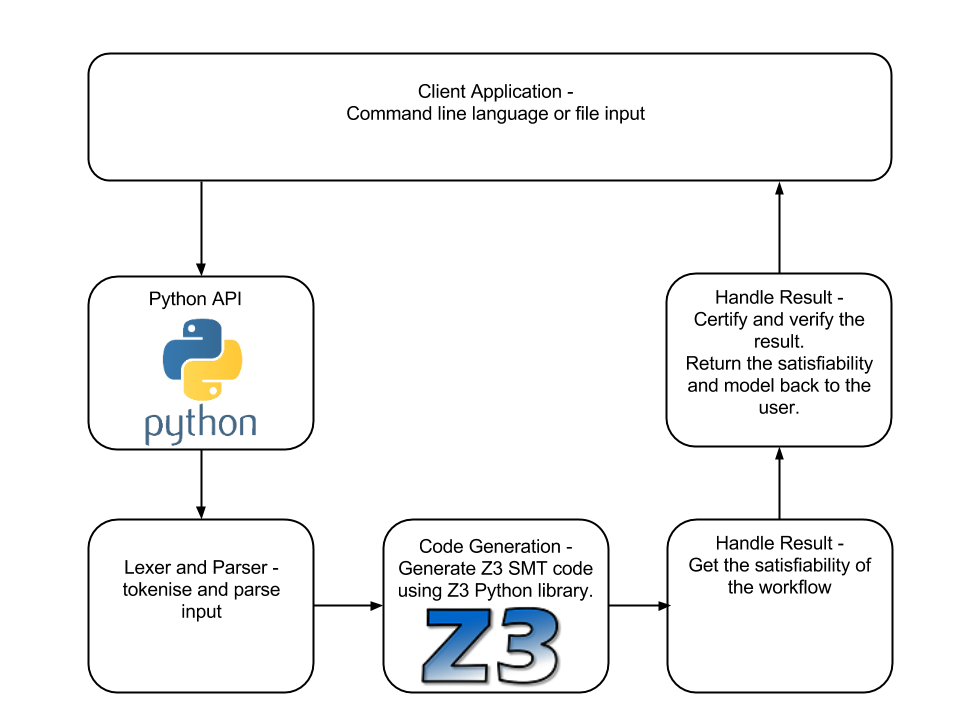
\includegraphics[scale=0.5]{ApplicationDiagram.png}
\caption{Application outline}
\label{fig:Application outline}
\end{figure}

\section{The Language}
Our requirements given was to design a language in which important constraints on the execution of tasks within a business process can be specified. It should be:
\begin{itemize}
\item easy to express workflows.
\item include temporal execution of tasks.
\item include separation of duty.
\item include binding of duty.
\item include constraints on allocation of tasks to users in the workflow.
\item include seniority.
\item include which users are authorised to execute which tasks.
\item include constraints to control the execution of the workflow.
\end{itemize} 

\subsection{Tasks and Users}
We have defined a basic language to fulfil these requirements. At first, the user must declare tasks and users within the domain of the workflow. In this example, the user has defined a list of tasks and users that are declared using \texttt{Tasks:} and \texttt{Users:} respectively. Following their declarations, is the list of tasks and users which are expressed using quotation marks and separated by commas. 
\lstset{numbers=none, showspaces=false,
    showstringspaces=false, tabsize=2, breaklines=true,
    xleftmargin=5.0ex,
}
\lstset{basicstyle=\ttfamily}
\begin{lstlisting}[frame=single]
Tasks: `receive_order', `price_large_order', 
	`price_small_order', `checkout'; 
Users: `alice', `bob', `carol';
\end{lstlisting}

\subsection{Separation of Duty}
We can then express different constraints on the workflow. To express separation of duty, we can use a keyword \texttt{SoD:} as the separation of duty declaration for all pairs of tasks. Each task expressed in each pair has to have different users. For the given example, whomever is allocated \texttt{receive\_order} must be different to the user who is allocated \texttt{checkout}.
\begin{lstlisting}[frame=single]
Tasks: `receive_order', `price_large_order', 
	`price_small_order', `checkout'; 
Users: `alice', `bob', `carol';
SoD: ('receive_order', 'checkout');
\end{lstlisting}

\subsection{Binding of Duty}
The constraint on binding of duty can be similarly expressed like separation of duty. The keyword for binding of duty is \texttt{BoD:} which delcares the list of pairs of tasks which must have the same user. In this example, whomever is allocated \texttt{price\_large\_order} must be the same user as the user who is allocated \texttt{price\_small\_order}.
\begin{lstlisting}[frame=single]
Tasks: `receive_order', `price_large_order', 
	`price_small_order', `checkout'; 
Users: `alice', `bob', `carol';
BoD: ('price_large_order', 'price_small_order');
\end{lstlisting}

\newpage

\subsection{Seniority}
There are many rules expressed using seniority. To express levels of seniority, we can again, give a list of pairs of users in this binary relation. The first user of their pair is more senior than the second user. We can use the keyword \texttt{Seniority:} to declare pairs of users who are senior to each other. In this example, we can see that Alice is more senior than Bob and Carol, and Bob is more senior than Carol.
\begin{lstlisting}[frame=single]
Tasks: `receive_order', `price_large_order', 
	`price_small_order', `checkout'; 
Users: `alice', `bob', `carol';
Seniority: (`alice', `bob'), (`alice', `carol'), (`bob', `carol');
\end{lstlisting} 


To use the seniority rules we have just specified, we can now set tasks to have relative seniority to other tasks within the workflow. These are given as single task options with \texttt{-min\_sec\_lv:} as an option flag, followed by a list of tasks.
\begin{lstlisting}[frame=single]
Tasks: `receive_order' -min_sec_lv:<[`price_large_order', `price_small_order', `checkout'], 
	`price_large_order' -min_sec_lv:>[`receive_order'] 
		-min_sec_lv:=[`price_small_order'], 
	`price_small_order' -min_sec_lv:>[`receive_order'] 
		-min_sec_lv:=[`price_large_order'], 
	`checkout' -min_sec_lv:>[`receive_order']; 
Users: `alice', `bob', `carol'; 
Seniority: (`alice', `bob'), (`alice', `carol'), (`bob', `carol');
\end{lstlisting} 

We can specify that tasks can be:
\begin{itemize}
\item equal seniority to another task. \\
\texttt{`price\_large\_order' -min\_sec\_lv:=[`price\_small\_order']}, so the task\\ \texttt{price\_large\_order} has to have a user that is equal seniority to whoever is allocated task \texttt{price\_small\_order}. In our case, this means that they are the same user. If we specified a constraint that they have to be different users, in our case, this would be a contradiction and the workflow would not be satisfied.
\item greater seniority to another task.\\ 
\texttt{`checkout' -min\_sec\_lv:>[`receive\_order'];}, so the task \texttt{checkout} has a minimum security level that it must be allocated a user that has a greater seniority than the user who is allocated the task \texttt{receive\_order}.
\item less seniority to another task.\\
\texttt{`receive\_order' -min\_sec\_lv:<[`price\_large\_order', `price\_small\_order',}\\ \texttt{`checkout']}, the task \texttt{receive\_order} has to be allocated a user that is less senior than the user who is allocated the task \texttt{price\_small\_order}.
\item not equal seniority to another task.\\
\texttt{`receive\_order' -min\_sec\_lv:!=[`price\_large\_order', `price\_small\_order', `checkout']}, the task \texttt{receive\_order} must not be the same seniority as the user allocated the task \texttt{price\_small\_order}. In our case, they would have to be separate users, so having a binding of duty rule specifying that \texttt{receive\_order} must be the same user as \texttt{price\_small\_order} produces a contradiction similarly to equal seniority.
\end{itemize}

\subsection{Worst Time to Completion}
We can express worst time completion by giving each task a duration time. This again is given as an option flag \texttt{-duration:} followed by the duration of the task. We can see in the example below that the task \texttt{receive\_order} has a duration of 50. This could be any unit of time and the user must account for this by making all their duration times the same unit.
\begin{center}
\begin{minipage}{\linewidth}
\begin{lstlisting}[frame=single]
Tasks: `receive_order' -duration:(50), 
	`price_large_order' -duration:(60), 
	`price_small_order' -duration:(100), 
	`checkout' -duration:(10); 
Users: `alice', `bob', `carol'; 
Seniority: (`alice', `bob'), (`alice', `carol'), (`bob', `carol');
\end{lstlisting}
\end{minipage}
\end{center}

\subsection{Temporal Order of Execution}
For expressing temporal order of execution, we can give a rule \texttt{Before:} which declares a list of pairs of tasks that have a before relationship. The first task of this pair is before the second task. In this example, the task \texttt{price\_large\_order} is executed before task \texttt{checkout}.
\begin{lstlisting}[frame=single]
Tasks: `receive_order', `price_large_order', 
	`price_small_order', `checkout'; 
Users: `alice', `bob', `carol';
Before: (`price_large_order', `checkout');
\end{lstlisting}

\subsection{Task Execution}
There are three different task executions: and, or and exclusive-or. We can specify each task execution rule with a rule \texttt{Execution:} with the following task execution. Since the default is an and execution, we must specify whether it will be an \texttt{Or} or \texttt{Xor} execution. Each task execution is followed by a pair \texttt{(t, [t\textsubscript{1},.., t\textsubscript{n}])}. In this example, we have specified an \texttt{Or} execution at the task \texttt{receive\_order}. Then, depending on any other constraints on the workflow, it can either execute \texttt{price\_large\_order} or \texttt{price\_small\_order} or both.
\begin{lstlisting}[frame=single]
Tasks: `receive_order', `price_large_order', 
	`price_small_order', `checkout'; 
Users: `alice', `bob', `carol';
Execution: Or(`receive_order', [`price_large_order', 
	`price_small_order']);
\end{lstlisting}

\subsection{Authorised Users}
We can give a list of users that are authorised to execute certain tasks and only those users. To declare authorised users to a task we can use the keyword \texttt{Authorised:}, followed by a pair, where the first of the pair is the task that is to be allocated, and the second is a list of users that are authorised to be allocated to that specific task. In this example, the only users that can be allocated the task \texttt{price\_large\_order} is \texttt{alice} and \texttt{bob}, but not \texttt{carol} as she has not been listed as an authorised user.
\begin{lstlisting} [frame=single]
Tasks: `receive_order', `price_large_order',
	`price_small_order', `checkout'; 
Users: `alice', `bob', `carol';
Authorised: (`price_large_order', [`alice', `bob'])
\end{lstlisting}

\section{Lexer and Parser} 
\subsection{PLY}
The interpreter is designed using PLY\cite{ply} (Python Lex-Yacc) which is a Python module. It is made up of two compiler construction tools: lex and yacc\cite{plylexyacc}. Yacc is ``Yet another compiler compiler'' and lex is the lexical analyser generator. The type of parsing used in PLY is LALR(1)\cite{lalr} Look-Ahead Left-Right parser.\\

We chose to use PLY rather than any other resources for tokenising, lexing and parsing because the library we are using for Z3 is a module for Python. This meant we had to choose a lexer and parser that is written in Python. PLY is a pure Python implementation of lex and yacc and uses a lot of python features that make it easy to use and well suited for our basic language. \\

We considered other lexers and parsers, but unfortunately, their specifications did not match with what we needed for this project:
\begin{itemize}
\item Antlr\cite{antlr} - It has a good lexer and parser with regular expressions. It generates a parsing tree visitor which is useful for code generation. However, the language that we have developed in this project is quite basic and does not need such complicated tools.
\item Pyparsing\cite{pyparsing} - It has an alternative approach to creating and executing simple grammars. It is different to traditional lex and yacc approach and does not use regular expressions. Therefore it may have been too heavy weight for this project. The main aim of this project is to focus on simple grammars with regular expressions.
\end{itemize}

\newpage

\subsection{Lexer}
The lexer uses the PLY lexer module. It takes in a list of tokens and reserved words that are exclusive to the language which the user is not allowed to use. We will later use these tokens and reserved words to apply parsing rules to them. Reserved words are keywords that are used in the syntax and the tokens are symbols.
We have a list of reserved words for the language:
\begin{itemize}
\item \texttt{Tasks} - Keyword to start the list of tasks
\item \texttt{Users} - Keyword to start the list of users
\item \texttt{Before} - Keyword to start the list of pairs of tasks temporal execution
\item \texttt{SoD} - Keyword to start the list of pairs of tasks that are bound to separation of duty
\item \texttt{Seniority} - Keyword to start the list of pairs of users that are senior to each other
\item \texttt{BoD} - Keyword to start the list of pairs of tasks that are bound to binding of duty
\item \texttt{min\_sec\_lv} - Keyword option for giving a minimum security level seniority for a task
\item \texttt{Or} - Keyword that decides the execution of a task by using an or-fork
\item \texttt{Xor} - Keyword that decided the execution of a task by using a xor-fork
\item \texttt{Execution} - Keyword option for the execution of tasks
\item \texttt{Authorised} - Keyword option for the list of users who are authorised to be allocated to a task
\item \texttt{duration} - Keyword option to state the duration of a task
\end{itemize}

We also have a list of tokens which uses regular expressions:
\begin{itemize}
\item \texttt{Colon} - : 
\item \texttt{Option} - -
\item \texttt{Comma} - ,
\item \texttt{LParen} - (
\item \texttt{RParen} - )
\item \texttt{End} - ;
\item \texttt{Eq} - =
\item \texttt{Lt} - $<$
\item \texttt{Gt} - $>$
\item \texttt{Neq} - !=
\item \texttt{LSqParen} - [
\item \texttt{RSqParen} - ]
\item \texttt{Number} - (decimal)  [0-9]+[\textbackslash.[0.9]+]?
\item \texttt{Node} - \say{(\textbackslash\textbackslash\ ``$|$[$\mathchar"5E$''])*}
\end{itemize}

\subsection{Parser}
As we have mentioned in this section earlier, PLY uses LALR(1) parsing. LALR(1) parsing is where a text is parsed according to a set of rules specified by a formal grammar.\\
We give an example of LALR(1) parsing:
\lstset{numbers=none, showspaces=false,
    showstringspaces=false, tabsize=2, breaklines=true,
    xleftmargin=5.0ex,
}
\begin{lstlisting}[frame=single]
begin : TASKS COLON task_node USERS COLON user_node
      | TASKS COLON task_node USERS COLON user_node rules
\end{lstlisting}

The grammar symbols (terminals) are represented using capital letters such as \texttt{TASKS}, \texttt{COLON}, \texttt{USERS} e.t.c. The grammar rules or identifiers (non-terminals) are expressed in lower case such as \texttt{task\_node}, \texttt{user\_node}, \texttt{rules}. They are made up of other non-terminals and terminals.\\	

The semantic behaviour of a language is defined by syntax directed translation, where there is a rule and action for each grammar symbol. We can give an example of the language:
\lstset{numbers=none, showspaces=false,
    showstringspaces=false, tabsize=2, breaklines=true,
    xleftmargin=5.0ex,
}
\begin{lstlisting}[frame=single]
Tasks: `receive_order', `price_large_order', 
`price_small_order', `checkout'; 
Users: `alice', `bob', `carol';
\end{lstlisting}

The keywords \texttt{Tasks}, \texttt{Users}, \texttt{:}, \texttt{;} and \texttt{,} are all terminals and are shifted when parsing as they do not have any grammar rules. However, the non-terminals such as \texttt{`receive\_order'} and \texttt{`alice'} have grammar rules associated to them and are reduced to the rules \texttt{task\_node} and \texttt{user\_node} respectively. \\

In the example, we have given a list of tasks, which are separated by a comma, \texttt{`receive\_order'} is reduced to a \texttt{NODE} terminal, the comma \texttt{,} is then reduced to the comma, which matched the second rule in \texttt{task\_node}. The next part of the rule is \texttt{task\_node} which recurses the \texttt{task\_node} rule and again, reduces the next task node \texttt{`price\_large\_order'} and so on. When we reach the last task node \texttt{`checkout'}, we reach the first rule \texttt{`end'}. The parser then goes to the end rule and reduces the \texttt{END} terminal as \texttt{;}. We can see that we have reached the end of the \texttt{task\_node} rule and is finally reduced to a \texttt{task\_node} non-terminal. A similar process is done when we reach the non-terminal \texttt{user\_node}. When the list of users is reduced to a \texttt{user\_node}, the rule is then reduced to the non-terminal \texttt{begin}. The whole input has been parsed as the first rule in \texttt{begin}.
\begin{lstlisting}[frame=single]
task_node : NODE end
          | NODE COMMA task_node
          | NODE variable_task_option
user_node : NODE end
          | NODE COMMA user_node
          | NODE user_option
          | NODE end_rule
end : END
    | END begin
\end{lstlisting}

PLY does some error handling for the lexer and parser\\
%TODO

As the input is being parsed, reduced and shifted, these are being added to a symbol table ready to generate the correct code. The symbol table is made up of dictionaries, where each entry has a key and value. The key is the task or user that we have applied a rule on, and the value is a list of tasks or users that are used within the rule. \\

\section{Code Generation}
We need to be able to generate the correct code so that we can parse it to Z3 correctly to get the satisfiability of the workflow as well as the model if applicable. Not only must we generate the correct code, but we have to have to correct axioms for each of the rules we have specified in the language that we do not need the user to know about or explicitly input.\\

The code is generated in such a way to make sure the ordering complies with Z3. We must declare all sorts before using them to define functions and constants in the theory. So in this implementation, it is best to declare all the sorts first, \texttt{Tasks} and \texttt{Users}. This gets rid of any unexpected sorts that Z3 might not recognise and return an error. We can then safely declare functions and constants with the correct types and finally any rules and axioms that are in that push-pop frame.\\

\subsection{Before Axioms}
%transitivity, cyclic
Since a workflow is an acyclic and directed graph, tasks cannot have any cycles. This is an applicable axiom as a task that has been executed cannot be executed again in our case. This makes defining workflows a lot easier. 
\begin{center}
$\forall t : Tasks (\neg before(t, t))$
\end{center}
\begin{lstlisting}[frame=single]
(assert (forall ((t Task))
(not (before t t))))
\end{lstlisting}

The \texttt{before} function is also transitive. 

\begin{center}
$\forall t, t\ensuremath{'}, t\ensuremath{''}  : Task (before(t, t\ensuremath{'}) \wedge before(t\ensuremath{'}, t\ensuremath{''})) \longrightarrow before(t, t\ensuremath{''})$
\end{center}

\begin{lstlisting}[frame=single]
(assert (forall ((t1 Task) (t2 Task) (t3 Task))
(=> (and (before t1 t2) (before t2 t3))
(before t1 t3))))
\end{lstlisting}

\subsection{Seniority Axioms}
The \texttt{seniority} function is transitive as it is a hierarchy.\\
\begin{center}
$\forall u, u\ensuremath{'}, u\ensuremath{''}  : User (seniority(u, u\ensuremath{'}) \wedge seniority(u\ensuremath{'}, u\ensuremath{''})) \longrightarrow seniority(u, u\ensuremath{''})$
\end{center}
\begin{lstlisting}[frame=single]
(assert (forall ((u1 User) (u2 User) (u3 User)) 
(=> (and (seniority u1 u2) (seniority u2 u3)) 
(seniority u1 u3))))
\end{lstlisting} 

This function is also acyclic because in a business, there cannot be a user who is both senior and junior to another user in the domain, so therefore they cannot be senior to themselves.
\begin{center}
$\forall u : User (\neg seniority(u, u))$
\end{center}
\begin{lstlisting}[frame=single]
(assert (forall ((u User))
(not (seniority u u))))
\end{lstlisting}

We take note that the \texttt{seniority} function is not relational. For example, if we have:
\begin{itemize}
\item $seniority(alice, bob)$
\item $seniority(bob, david)$
\item $seniority(carol, david)$
\end{itemize}
We have the seniority diagram as:
\begin{figure}[!h]
\center
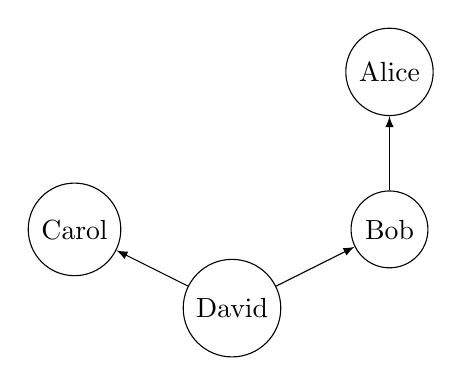
\begin{tikzpicture}
\tikzset{vertex/.style = {shape=circle,draw,minimum size=1.5em}}
\tikzset{edge/.style = {->,> = latex}} 
%\draw (0,0) circle [radius=0.5];
\node[vertex] (a) at  (0,0) {Carol};
\node[vertex] (b) at  (4,2) {Alice};
\node[vertex] (c) at (2,-1) {David};
\node[vertex] (d) at (4,0) {Bob};
\draw[edge] (c) to (a);
\draw[edge] (c) to (d);
\draw[edge] (d) to (b);
\end{tikzpicture}
\end{figure}

By not being relational, we cannot deduce that Bob and Carol are on the same level of seniority as each other since Alice is only senior to Bob and not senior to Carol. Therefore in our model, we express having the same seniority means that the user has to be the same user. Similarly to having different levels of seniority, it must just be the case that they are different users since \texttt{seniority} is not relational.\\

If we wanted to express that Carol and Bob were on the same seniority level, Alice would also need to be senior to Carol $seniority(alice, carol)$
\begin{center}
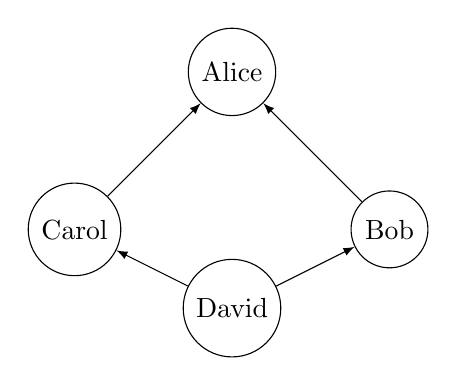
\begin{tikzpicture}
\tikzset{vertex/.style = {shape=circle,draw,minimum size=1.5em}}
\tikzset{edge/.style = {->,> = latex}} 
%\draw (0,0) circle [radius=0.5];
\node[vertex] (a) at  (0,0) {Carol};
\node[vertex] (b) at  (2,2) {Alice};
\node[vertex] (c) at (2,-1) {David};
\node[vertex] (d) at (4,0) {Bob};
\draw[edge] (c) to (a);
\draw[edge] (c) to (d);
\draw[edge] (d) to (b);
\draw[edge] (a) to (b);
\end{tikzpicture}
\end{center}

\subsection{Execution of Tasks in Worflows}
In the workflow, the user can define different forms of forking: and, or and exclusive-or. This means that there are different possibilities of tasks which are actually allocated and therefore executed in the workflow. For example, if we have a separation of duty within a workflow and there is an or fork before this constraint, we might not need to actually execute those tasks under that constraint. An example of this workflow is given in Figure~\ref{fig:Over constrained workflow}. The dotted lines show the tasks that are constrained under separation of duty, $SoD(t_2, t_3)$ and $SoD(t_2, t_4)$. So if task $t_3$ is chosen to execute as task $t_2$ cannot be allocated or would be unsatisfied, then we do not need to worry about the separation of duty constraints in place as those tasks under it are never executed, $SoD(t_2, t_3)$ and $SoD(t_2, t_4)$ as $t_2$ was never executed. This means that we do not need to over constrain the workflow, making task allocation easier.
\begin{figure}[!htb]
\centering
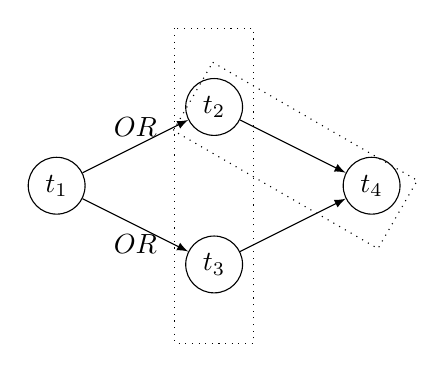
\begin{tikzpicture}[cloud/.style={
      draw=black,
      thick,
      ellipse,
      fill=red!20,
      minimum height=2em
    }]
\tikzset{vertex/.style = {shape=circle,draw,minimum size=1.5em}}
\tikzset{edge/.style = {->,> = latex}} 
%\draw (0,0) circle [radius=0.5];
\node[vertex] (a) at  (0,0) {$t_{1}$};
\node[vertex] (b) at  (2,1) {$t_{2}$};
\node[vertex] (c) at (2,-1) {$t_{3}$};
\node[vertex] (d) at (4,0) {$t_{4}$};
\draw[edge] (b) to (d);
\draw[edge] (c) to (d);
\path[-latex]
(a) edge node[above] {$OR$} (b)
(a) edge node[below] {$OR$} (c);
\draw[dotted] (1.5,2) rectangle (2.5,-2);
\draw[dotted, rotate around={60:(0.5,3)}] (0,1) rectangle (-1,-2);
\end{tikzpicture}
\caption{Over constrained workflow}
\label{fig:Over constrained workflow}
\end{figure}

We introduce an auxiliary user ``bottom'' who a user and is allocated tasks which cannot be executed. This is an in-system user who has been predeclared without the user explicitly listing it. Therefore the user can never inout a user in the universe called `bottom'.
\begin{lstlisting}[frame=single]
(declare-const bottom User)
\end{lstlisting}

We must ensure that all the input users are different to bottom, otherwise bottom could be allocated to tasks which actual users in the domain could be allocated to. We need to keep this separate. So we make sure that all users in the domain must be more senior than bottom:
\begin{center}
$\forall u : User ((u \neq bottom) \longrightarrow ((\neg seniority(bottom, u) \wedge (\neg seniority(u, bottom))))$
\end{center}
\begin{lstlisting}[frame=single]
(assert (forall ((u User))
(=>(not(= u bottom))
(and (not(seniority bottom u)) (not(seniority u bottom))))))
\end{lstlisting}

But \texttt{bottom} must be able to be allocated to other tasks in the case that the particular task is not executable:
\begin{center}
$alloc\_user(t) = bottom$
\end{center}
\begin{lstlisting}[frame=single]
(assert(=(alloc_user t) bottom))
\end{lstlisting}

Firstly, we have to make sure that if a task is executed, that it is not allocated to the bottom user. This is due to the bottom user is as a user who is allocated all the unallocated tasks.
\begin{center}
$\forall t : Task (executed(t) \longrightarrow ( alloc\_user(t) \neq bottom))$
\end{center}
\begin{lstlisting}[frame=single]
(assert (forall ((t Task))
(=> (executed t)
(not(=(alloc_user t) bottom)))))
\end{lstlisting}

We have to also make sure that all the not executed tasks are allocated to the bottom user. 
\begin{center}
$\forall t : Task (\neg executed(t) \longrightarrow (alloc\_user(t) = bottom))$
\end{center}
\begin{lstlisting}[frame=single]
(assert (forall ((t Task))
(=> (not(executed t))
(=(alloc_user t) bottom)))
\end{lstlisting}

With these axioms in place, we can make sure that only the executed tasks are allocated to the domain of given users and the executed tasks are allocated to the bottom user. So now we must  wrap all our previous axioms and rules with the executed axiom.\\

For the seniority rules and axioms, we must wrap them with the execution rule so that we know which tasks are executed and allocatable to the domain of users, and which tasks are not. \\

For two tasks to be executed by users of the same seniority (the same user):
\begin{center}
$(executed(t) \wedge executed(t\ensuremath{'})) \longrightarrow (alloc\_user(t) = alloc\_user(t\ensuremath{'}))$
\end{center}
\begin{lstlisting}[frame=single]
(assert 
(=>(and (executed t) (executed t'))
(=(alloc_user t) (alloc_user t'))))
\end{lstlisting}

Similarly to two tasks having to have the same level of seniority. When two tasks have different seniority, they have to have different users:
\begin{center}
$(executed(t) \wedge executed(t\ensuremath{'}) \longrightarrow (alloc\_user(t) \neq alloc\_user(t\ensuremath{'})))$
\end{center}

\begin{lstlisting}[frame=single]
(assert 
(=>(and (executed t) (executed t'))
(not(=(alloc_user t) (alloc_user t')))))
\end{lstlisting}

Greater and less than seniority are shown below respectively where \texttt{(assert (seniority t t'))}
\begin{center}
$(executed(t) \wedge executed(t\ensuremath{'})) \longrightarrow seniority(alloc\_user(t), alloc\_user(t\ensuremath{'})$
\end{center}
\begin{lstlisting}[frame=single]
(assert 
(=> (and (executed t) (executed t'))
(seniority (alloc_user t) (alloc_user t'))))
\end{lstlisting}
\begin{center}
$(executed(t) \wedge executed(t\ensuremath{'})) \longrightarrow seniority(alloc\_user(t\ensuremath{'}), alloc\_user(t)$
\end{center}
\begin{lstlisting}[frame=single]
(assert 
(=>(and (executed t') (executed t))
(seniority (alloc_user t') (alloc_user t))))
\end{lstlisting}

We also need to wrap separation of duty and binding of duty around an executed rule which are shown below respectively. 
\begin{center}
$(executed(t) \wedge executed(t\ensuremath{'})) \longrightarrow (alloc\_user(t) \neq alloc\_user(t\ensuremath{'}))$
\end{center}
\begin{lstlisting}[frame=single]
(assert 
(=> (and (executed t) (executed t'))
(not (=(alloc_user t) (alloc_user t')))))
\end{lstlisting}
\begin{center}
$(executed(t) \wedge executed(t\ensuremath{'})) \longrightarrow (alloc\_user(t) = alloc\_user(t\ensuremath{'}))$
\end{center}
\begin{lstlisting}[frame=single]
(assert 
(=> (and (executed t) (executed t'))
(=(alloc_user t) (alloc_user t'))))
\end{lstlisting}

\subsection{Unique Users}
%neq bottom, unique users axiom, 
We have to ensure that all users are unique from each other. Z3 may not be able to execute some of the axioms and it may not be able to tell users apart and therefore not be able to allocate users to tasks. We have provided two axioms to solve this issue: to explicitly declare that each user is unique to each other and that they are the only users in the set, and therefore the only users in the universe.\\

To declare that all users are unique to each other, where $u, u\ensuremath{'} \in Users$:
\begin{center}
$u \neq u\ensuremath{'}$
\end{center}
\begin{lstlisting}[frame=single]
(assert (not(= u u')))
\end{lstlisting}

To declare that the users listed are the only users in the universe including the \texttt{bottom} user, where $u, u\ensuremath{'}, u\ensuremath{''} \in Users$: 
\begin{center}
$\forall u, u\ensuremath{'} : User ((u = u\ensuremath{'}) \vee (u = u\ensuremath{''}))$
\end{center}
\begin{lstlisting}[frame=single]
(assert (forall ((u User)) 
(or (= u u') (= u u''))))
\end{lstlisting}

\subsection{Worst Time Completion}
Another feature we included in this tool is to generate the worst time completion of a workflow. We need to generate this at the end after we check if the workflow is satisfiable. If it's unsatisfiable, then there is no need to check the worst time to completion as the workflow is not completed.\\

At first, we need to declare a constant that can represent the worst time in the workflow. The constant is a \texttt{Real} as the duration could possibly be an integer or a decimal. 
\begin{lstlisting}[frame=single]
(declare-const completion_time Real)
\end{lstlisting}

To obtain the completion time, we need to only sum the duration of all the tasks that have been executed in the workflow. To do this in Z3, we need to check each of the tasks in the workflow to see if they have been executed. If they have been executed, then they should be summed, otherwise, they should not be in the sum. To achieve this, we need to use an ``if-then-else'' (\texttt{ite}). If they are executed, then sum up the tasks' duration time, otherwise it's duration time should be zero as a task that has not been executed has no duration time in the satisfied workflow.
\begin{center}
$completion\ time = \sum\nolimits_{executed(t) = true} duration(t)$
\end{center}

\begin{lstlisting}[frame=single]
(assert (= completion_time
(+ (ite (executed t) (duration t) 0)...
   (ite (executed tn (duration tn) 0)))))"
\end{lstlisting}

Now that we have a completion time, we can write an algorithm that will do an unbounded search on the worst time completion, which is shown in Figure~\ref{fig:Unbound search}. We pass the completion time through as a parameter in Z3 with \texttt{delta} which is the limit where the algorithm will stop the bisection. To find the upper bound time, we keep checking that the completion time can be greater than double the models completion time. When we reach this point, we know that there is no longer a time where it could be worse and therefore we have reached the upper bound completion time. \\

\begin{figure}[h]
\center
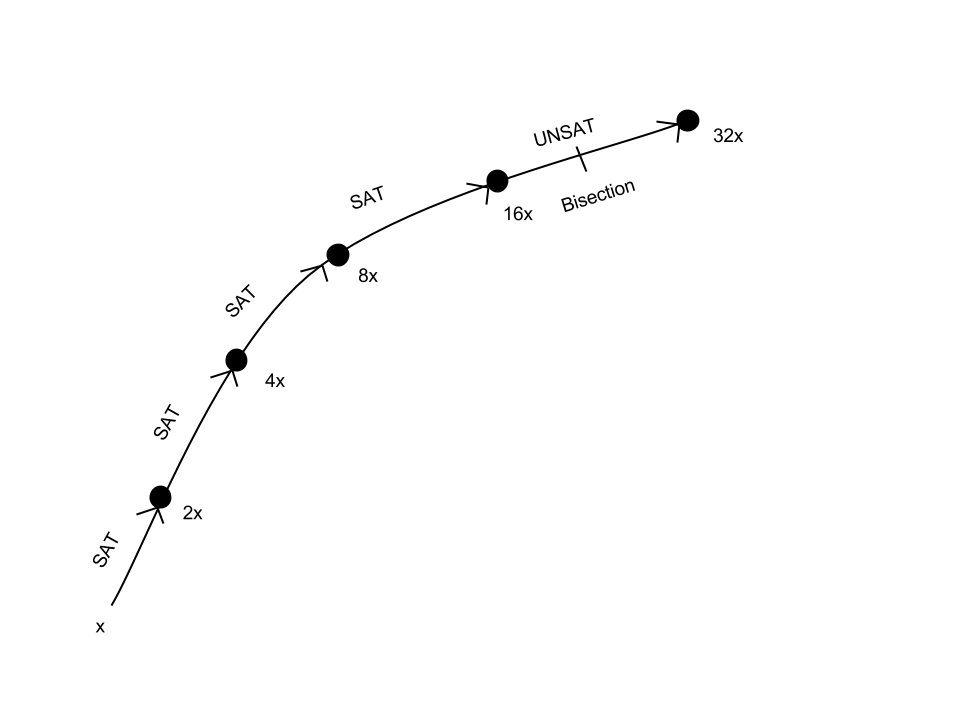
\includegraphics[scale=0.30]{UnboundSearch.png}
\caption{Unbound search}
\label{fig:Unbound search}
\end{figure}

Once we have the upper bound and the lower bound completion times we can begin the bisection. If the completion time is greater than the bisection of the upper and lower bounds, then the lower bound completion time should be set as the value of the bisection. However, if it's unsatisfiable, it means there is no completion time greater than the value of the bisection, so we must search the lower half of the bisection, setting the upper bound to the value of the bisection. We recurse though this bisection until we reach the bijection limit \texttt{delta}. We have then found the worst time completion as the midpoint of the two bounds. The algorithm is shown in Figure~\ref{fig:Worst Time Completion} \\
\[
\frac{upperbound + lowerbound}{2}
\]

\begin{figure}[H]
\lstset{numbers=left, showspaces=false,
    showstringspaces=false, tabsize=2, breaklines=true,
    xleftmargin=5.0ex,
}
\begin{lstlisting}[frame=single]
def worst_time_completion(x, delta, s):
	res = s.check()
	if res == unsat:
		return unsat
	else:
		m = s.model()
	# Finding the upper bound time
	x_s = Real(x)
	# Unbounded search
	while res == sat:
		s.push()
		s.add(x_s > 2*m[x_s])
		res = s.check()
		if res == sat:
			m = s.model()
		s.pop()
	# Bisection
	v = m[x_s]
	v = float(v.as_decimal(10)[:])
	max_time = 2*v
	min_time = v
	while (max_time-min_time) > delta:
		s.push()
		s.add((((max_time - min_time)/2)+min_time) <= x_s)
		res = s.check()
		if res == sat:
			min_time = (((max_time-min_time)/2)+min_time)
		else:
			max_time = (((max_time-min_time)/2)+min_time)
		s.pop()
	y = (max_time+min_time)/2
	return y 
\end{lstlisting}
\caption{Worst time completion}
\label{fig:Worst Time Completion}
\end{figure}

\section{Validation and Completeness of Z3 Model}
We need to be able to verify the completeness of the model with the actual input from the user. There could be the case the model returned from Z3 my be inconsistent even though the allocation returned back to the user may be correct. The application verifies four different aspects: separation of duty, binding of duty, seniority and lower bound worst time completion. We must check all combinations of user allocations, not including the bottom user as it is able to be allocated to all tasks, to check whether they are supposed to return satisfiable or unsatisfiable within the workflow.\\

\subsection{Separation of Duty}
To verify separation of duty of all tasks, we need to check that each pair of users that are allocated to the tasks that are under the constraint of separation of duty are not the same. We use the push-pop frame to test each allocation by pushing the stack and popping the stack when we have received the result so we can continue to test other users. \\

In Figure~\ref{Verification of separation of duty}, if the model itself is unsatisfied, then the verification fails and should return \texttt{false} as we cannot verify anything with an unsatisfied model. If it is satisfied, we can carry on the verification. We take each of the tasks in the separation of duty dictionary and we verify that each one is executed and that the users can be allocated the tasks. The result determines whether the model is consistent with the input. If the users are both the same and the result from \texttt{s.check()} is \texttt{sat} the verification should fail as the users who are allocated to the tasks should be different. Similarly, if the users are different and the result from the check is \texttt{unsat}, there must be some other constraint that is making this pair of users fail the verification. So we examine rules of seniority as a possibility of the failure to satisfy the allocation to the workflow. 

\begin{figure}[H]
\lstset{numbers=left, showspaces=false,
    showstringspaces=false, tabsize=2, breaklines=true,
    xleftmargin=5.0ex,
}
\begin{lstlisting}[frame=single]
def verify_result_sod(original, s, u):
	verify_original = original[:]
	verify = True
	s.push()
	res = s.check()
	if res == unsat:
		verify = False
		return verify
	for sod in dict_sod:
		v = z3.parse_smt2_string(verify_original)
		s.add(v)
		s.push()
		verify_original += "(push)\n"
		verify_original += "(assert (and (executed " + sod[0] +") (= (alloc_user " + sod[0] +")" + u[0] + ")))\n"
		verify_original += "(assert (and (executed " + sod[1] +") (= (alloc_user " + sod[1] +")" + u[1] + ")))\n"
		v = z3.parse_smt2_string(verify_original)
		s.add(v)
		if u[0] == u[1]:
			if s.check() == sat:
				verify = False
				s.pop()
				verify_original += "(pop)\n"
			else:
				s.pop()
				verify_original += "(pop)\n"
		elif u[0] != u[1]:
			if s.check() == sat:
				s.pop()
				verify_original += "(pop)\n"
			else:
				s.pop()
				verify = self.verify_result_seniority(original, s, u)
				verify_original += "(pop)\n"
	return verify
\end{lstlisting}
\caption{Verification of separation of duty}
\label{Verification of separation of duty}
\end{figure}

\newpage

\subsection{Binding of Duty}
Similarly to separation of duty, we must check the equality of the users that are allocated to the tasks that are listed in the binding of duty constraints.\\ 

In Figure~\ref{fig:Verification of binding of duty}, if the users are not the same and \texttt{s.check()} returns \texttt{unsat}, then it is breaking the binding of duty constraint and the verification should fail. However, if they are both the same user, then it should be \texttt{sat}. But if it is \texttt{unsat}, there may be another constraint on that pair of users being allocated those particular tasks. We check any seniority constraints to check the validity of the pair of users being allocated to the tasks.\\

\begin{figure}[!h]
\lstset{numbers=left, showspaces=false,
    showstringspaces=false, tabsize=2, breaklines=true,
    xleftmargin=5.0ex,
}
\begin{lstlisting}[frame=single]
def verify_result_bod(original, s, u):
	verify_original = original[:]
	verify = True
	s.push()
	for bod in dict_bod:
		v = z3.parse_smt2_string(verify_original)
		s.add(v)
		s.push()
		verify_original += "(push)\n"
		verify_original += "(assert (and (executed " + bod[0] +") (= (alloc_user " + bod[0] +")" + u[0] + ")))\n"
		verify_original += "(assert (and (executed " + bod[1] +") (= (alloc_user " + bod[1] +")" + u[1] + ")))\n"
		v = z3.parse_smt2_string(verify_original)
		s.add(v)
		if u[0] != u[1]:
			if s.check() == sat:
                    verify = False
		elif u[0] == u[1]:
			if s.check() == unsat:
				s.pop()
				verify = self.verify_result_seniority(original, s, u)
		s.pop()
		verify_original += "(pop)\n"
	return verify
\end{lstlisting}
\caption{Verification of binding of duty}
\label{fig:Verification of binding of duty}
\end{figure}

\newpage

\subsection{Seniority}
To check that all the users are valid with the seniority constraints, we need to check the different levels of security for each task with respect to other tasks. \\

We check every different constraint on the tasks as we have stored in our symbol table. For seniority constraints, we have a different dictionary for each type of security level. We test each level to make sure it complies with the user input and that it is not breaking any other constraints in the rule.\\

For two tasks to have equal levels of seniority they have to have the same user. So we do a similar check that we have done in separation of duty. Similarly with checking if two tasks having different levels of seniority, it is similar to the binding of duty verification. \\

When a task has to be allocated a user with greater seniority than another, we test if both tasks are executed with that particular allocation. If the result is \texttt{unsat} but the first user in the user pair is more senior which is compared to the seniority dictionary in the symbol table, then verification fails as it should be true. However, if the result from \texttt{s.check()} returns \texttt{sat} when the first user is less senior to the second in the user pair, verification should also fail. When a task has to be allocated to a user with less seniority than another, we check that the task which needs to be allocated the less senior user is allocated the second user of the pair. If \texttt{s.check()} returns \texttt{unsat}, we check that the seniority is correct with the seniority input in the symbol table. If the less senior user has been allocated the task that required a less senior user but the result was \texttt{unsat} then verification should fail. If the result was \texttt{sat}, then we need to test to make sure that the user allocated to the less senior task is in face less senior to the other user. If it is not, the verification should fail again.\\

\begin{figure}[H]
\lstset{numbers=left, showspaces=false,
    showstringspaces=false, tabsize=2, breaklines=true,
    xleftmargin=5.0ex,
}
\begin{lstlisting}[frame=single]
def verify_result_seniority(original, s, u):
	verify = True
	verify_original = original[:]
	if dict_seniority:
		for t_key, t_value in dict_eq_tasks.iteritems():
			s.push()
			verify_original += "(assert (= " + u[0] + " " + u[1] + "))"
			v = z3.parse_smt2_string(verify_original)
			s.add(v)
			if s.check() == unsat:
				if u[0] == u[1]: verify = False
			else:
				if u[0] != u[1]: verify = False
			s.pop()
		for t_key, t_value in dict_gt_tasks.iteritems():
			for v in t_value:
				s.push()
				verify_original += "(assert (and (executed " + t_key + ") \
					"(executed " + v + ")" \
					"(= (alloc_user " + t_key +")" + u[0] + ")" \
					"(= (alloc_user " + v + ")" + u[1] + ")))"
				v = z3.parse_smt2_string(verify_original)
				s.add(v)
				if s.check() == unsat:
					for u_key, u_value in dict_seniority.iteritems():
						if u[0] == u_key and u[1] in u_value: verify = False
						else:
							for u_key, u_value in dict_seniority.iteritems():
								if u[0] == u_key and u[1] not in u_value: 
									verify = False
				s.pop()  
		for t_key, t_value in dict_lt_tasks.iteritems():
			for v in t_value:
				s.push()
				verify_original += "(assert (and (executed " + t_key + ")" \
					"(executed " + v + ") " \
					"(= (alloc_user " + t_key +")" + u[1] + ")" \
					"(= (alloc_user " + v + ")" + u[0] + ")))"
				v = z3.parse_smt2_string(verify_original)
				s.add(v)
				if s.check() == unsat:
					for u_key, u_value in dict_seniority.iteritems():
						if u[0] == u_key and u[1] in u_value: verify = False
				else:
					for u_key, u_value in dict_seniority.iteritems():
						if u[0] == u_key and u[1] not in u_value: verify = False
				s.pop()
		if dict_neq_tasks:
			verify_original += "(assert(not(= " + u[0] +" "+ u[1] + ")))"
			v = z3.parse_smt2_string(verify_original)
			s.add(v)
			if s.check() == unsat:
				if u[0] != u[1]: verify = False
				else:
					if u[0] == u[1]: verify = False
			s.pop()
	return verify
\end{lstlisting}
\end{figure}

\subsection{Lower Bound Worst Time Completion}
When computing the worst time completion, we need to make sure that the lower bound of the worst time completion cannot get any lower otherwise the average we take between the upper and lower bound could be worse.

\begin{figure}[!h]
\lstset{numbers=left, showspaces=false,
    showstringspaces=false, tabsize=2, breaklines=true,
    xleftmargin=5.0ex,
}
\begin{lstlisting}[frame=single]
s.push()
	duration_total = 0
	dur_tot = Real('duration_total')
	Task = DeclareSort('Task')
		for ms in m:
			if "executed" in str(ms) and "!" not in str(ms):
				for ts in tasks:
					t = Const(ts, Task)
					for mss in m:
						if "duration" in str(mss):
							duration_total = duration_total + 
							m.eval(mss(t))
		s.add(dur_tot >= duration_total)
		if s.check() == unsat:
			return unsat
		s.pop()
\end{lstlisting}
\caption{Verifying worst time completion}
\label{fig:Verifying worst time completion}
\end{figure}

To verify that there are no executions of tasks which fall below the lower bound and that the lower bound calculated is truly the lower bound we check the model returned using \texttt{s.model()}, shown in Figure~\ref{fig:Verifying worst time completion}. We check that if the task is executed, the sum of the duration time must be above the lower bound. If the total durations of all the executed tasks are less than the lower bound, then the lower bound we have calculated may not be correct and we should return \texttt{unsat},otherwise we should return the worst time completion. \\

\section{Handling The Result}
Z3 has a API method call \texttt{model()} which returns a model back to the user. However, this model can be quite hard to read. With a huge workflow with many tasks and users, the universe it reports back will include all the constants and function mappings. In Figure~\ref{fig:Command line worflow input} we can see the user input of a workflow and in Figure~\ref{fig:Z3 API model output} the original Z3 model output. 

\begin{figure}[H]
\centering
\begin{subfigure}[b]{\textwidth}
\begin{lstlisting}[frame=single]
Tasks: 'receive_order' -min_sec_lv:<['price_large_order', 'price_small_order', 'checkout'] -duration:(50), 'price_large_order' -min_sec_lv:>['receive_order'] -min_sec_lv:=['price_small_order'] -duration:(10), 'price_small_order' -min_sec_lv:>['receive_order'] -min_sec_lv:=['price_large_order'] -duration:(100), 'checkout' -min_sec_lv:>['receive_order'] -duration:(10); Users: 'alice', 'bob', 'carol'; Seniority: ('alice', 'bob'), ('alice', 'carol'), ('bob', 'carol');
\end{lstlisting}
\caption{Command line workflow input}
\label{fig:Command line worflow input}
\end{subfigure} \\
\begin{subfigure}[b]{\textwidth}
\begin{lstlisting}[frame=single]
[receive_order = Task!val!2,
 completion_time = 170,
 price_large_order = Task!val!3,
 alice = User!val!3,
 elem!60 = Task!val!4,
 price_small_order = Task!val!0,
 bottom = User!val!0,
 checkout = Task!val!1,
 bob = User!val!1,
 carol = User!val!2,
 elem!908 = Task!val!2,
 before = [else -> False],
 executed = [else -> True],
 alloc_user = [else -> alloc_user!913(k!911(Var(0)))],
 seniority = [else ->
              seniority!914(k!910(Var(0)), k!910(Var(1)))],
 k!911 = [Task!val!1 -> Task!val!1,
          Task!val!2 -> Task!val!2,
          Task!val!3 -> Task!val!3,
          Task!val!4 -> Task!val!4,
          else -> Task!val!0],
 duration = [Task!val!0 -> 100,
             Task!val!2 -> 50,
             else -> 10],
 k!910 = [User!val!3 -> User!val!3,
          User!val!0 -> User!val!0,
          User!val!1 -> User!val!1,
          else -> User!val!2],
 alloc_user!913 = [Task!val!2 -> User!val!2,
                   else -> User!val!3],
 seniority!914 = [(User!val!1, User!val!2) -> True,
                  (User!val!3, User!val!1) -> True,
                  (User!val!3, User!val!2) -> True,
                  else -> False]]
\end{lstlisting}
\caption{Z3 API model output}
\label{fig:Z3 API model output}
\end{subfigure}
\caption{Z3 model result}
\label{fig:Z3 model result}
\end{figure}

\newpage

\subsection{Making It Human Readable}
We need to make this output more human readable as it is difficult to map constants to functions, especially if the universe is much larger than the example given in Figure~\ref{fig:Z3 model result}. We can automate this mapping as we finish the verification and give the output to the user. \\

As shown in Figure~\ref{fig:Making the model more human readable}, we map the users and tasks to the corresponding Z3 declarations so it is easier to translate the model as Z3 uses their own declarations rather than the actual user and task names. We then loop through the model looking for each function and passing tasks or users to the relavent parameters of the function and use them to evaluate the function. If the function returns \texttt{True}, then we can append it to the final result dictionary. \\

Finally after going through the entire model, we piece together the final result with all the functions. Each function has their result translated back into the appropriate task and user names and combined to return one final output. As seen in Figure~\ref{fig:Human readable output}, we have a list of seniority pairs from \texttt{seniority} which is consistent with the user input. We also have the list of allocated users to tasks \texttt{alloc\_user} of which those are executed. The list of executed tasks is also returned back to the user \texttt{executed\_tasks}, as well as the worst time completion and the list of tasks which where given by the user in \texttt{before}.

\begin{figure}[!h]
\begin{lstlisting}[frame=single]
{'seniority': [('bob', 'carol'), ('alice', 'carol'), ('alice', 'bob')], 'alloc_user': [[(carol, receive_order), (alice, price_small_order), (alice, checkout), (alice, price_large_order)]], 'executed_tasks': [receive_order, price_small_order, checkout, price_large_order], 'worst time completion': 170.0, 'before': []}
\end{lstlisting}
\caption{Human readable output}
\label{fig:Human readable output}
\end{figure}

\begin{figure}[H]
\lstset{numbers=left, showspaces=false,
    showstringspaces=false, tabsize=2, breaklines=true,
    xleftmargin=5.0ex,
}
\begin{lstlisting}[frame=single]
def evaluate_final_model(model, total_worst_duration):
	model_user_map = { }
	model_task_map = { }
	model_list = []
	model_result_map = { }
	Task = DeclareSort('Task')
	User = DeclareSort('User')
	for ms in model:
		if str(ms) in users:
			model_user_map[ms] = model[ms]
		if str(ms) in tasks:
			model_task_map[ms] = model[ms]
		if "before" in str(ms):
			before_task_list = []
			for t in itertools.product(tasks, tasks):
				t1 = Const(str(t[0]), Task)
				t2 = Const(str(t[1]), Task)
				before_tasks = model.eval(ms(t1, t2))
				if str(before_tasks) == "True":
					before_task_list.append(t)
			model_result_map["before"] = before_task_list
		if "alloc_user" in str(ms):
			model_list_list = []
			for t_key, t_value in model_task_map.iteritems():
				t = Const(str(t_key), Task)
				user_solution = model.eval(ms(t))
				for u_key, u_value in model_user_map.iteritems():
					if str(u_value) == str(user_solution):
						model_list_list.append((u_key, t_key))
			if model_list_list not in model_list:
				model_list.append(model_list_list)
				model_result_map["alloc_user"] = model_list
		if "executed" in str(ms):
			executed_task_list = []
			for t_key, t_value in model_task_map.iteritems():
				t = Const(str(t_key), Task)
				executed_task = model.eval(ms(t))
				if executed_task:
					executed_task_list.append(t_key)
					model_result_map["executed_tasks"] = executed_task_list
		if "seniority" in str(ms) and "!" not in str(ms):
			senior_users_list = []
			for u in itertools.product(users, users):
				u1 = Const(str(u[0]), User)
				u2 = Const(str(u[1]), User)
				senior_users = model.eval(ms(u1, u2))
				if str(senior_users) == "True":
					senior_users_list.append(u)
			model_result_map["seniority"] = senior_users_list
	model_result_map["worst time completion"] = round(total_worst_duration)
	return model_result_map
\end{lstlisting}
\caption{Making the model more human readable}
\label{fig:Making the model more human readable}
\end{figure}

\section{Unsatisfiable Core}
In this report, we have talked about the satisfied core as we are interested in whether the workflow is satisfied or unsatisfied. However, it is interesting to see which assertions do fail if the workflow is unsatisfied. In Z3 we call the method \texttt{get-unsat-core}. We also need to set the SMT flag \texttt{(set-option :produce-unsat-cores true)} to make sure that we can report the unsat core. To label each constraint in SMT, we wrap each assertion with \texttt{!(constraint):named x} where x is the label. This is shown in Figure~\ref{fig:Z3 unsatisfied core}. \\

The unsatisfied core reports which assertions are false within the given model. In order to state which assertions are being broken, we must label each one using \texttt{solver.assert\_and\_track(constraint, label)}. The label is the name we give to each assertion, so when we call \texttt{(solver.unsat\_core())} we should get back an empty array \texttt{[]} if the theory is satisfied, or a list of labels of assertions that are false. \\

If our workflow is unsatisfiable, for example if we set the constraints as the task \texttt{checkout} has to be allocated a user who has less seniority than whomever is allocated the task \texttt{receive\_order}. But we also have a constraint that whomever is allocated the task \texttt{receive\_order} has to be less senior than the user chosen to be allocated the task \texttt{checkout}. As seen in Figure~\ref{fig:Z3 unsatisfied core result}, we can see that the violated constraints are:
\begin{itemize}
\item  \texttt{(assert (! (=>(and (executed receive\_order) (executed checkout))\\
(seniority (alloc\_user receive\_order) (alloc\_user checkout)))\\
:named lttask0))}
\item \texttt{(assert (! (=>(and (executed checkout) (executed receive\_order))\\
(seniority (alloc\_user checkout) (alloc\_user receive\_order))) \\
:named lttask1))}
\item \texttt{(assert (! (executed receive\_order) :named a3))}
\item \texttt{(assert (! (executed checkout) :named a0))}
\end{itemize}
Which is consistent to our input.

\begin{figure}[!h]
\centering
\begin{subfigure}[b]{\textwidth}
\begin{lstlisting}[frame=single]
(set-option :produce-unsat-cores true)
(declare-sort Task) (declare-sort User) 
(declare-fun executed (Task) Bool)
(declare-fun before (Task Task) Bool) 
(declare-fun seniority (User User) Bool) 
(declare-const bottom User) 
(declare-fun alloc_user (Task) User) 
(declare-fun duration (Task) Real)
(assert (forall ((t1 Task) (t2 Task) (t3 Task))(=>(and(before t1 t2) (before t2 t3))(before t1 t3))))
(assert (forall ((u1 User) (u2 User) (u3 User)) (=> (and (seniority u1 u2) (seniority u2 u3)) (seniority u1 u3))))
(assert (forall ((u User))(=>(not(= u bottom))(and (not(seniority bottom u)) (not(seniority u bottom))))))
(assert (forall ((t Task))(not (before t t))))
(assert (forall ((u User))(not (seniority u u))))
(declare-const carol User) 
(declare-const bob User) 
(declare-const alice User) 
(declare-const checkout Task)
(declare-const price_small_order Task)
(declare-const price_large_order Task)
(declare-const receive_order Task)
(assert (forall ((t Task))(=> (executed t)(not(=(alloc_user t) bottom)))))
(assert (forall ((t Task))(=> (not(executed t))(=(alloc_user t) bottom))))
(assert (! (seniority bob carol) :named seniority0)) 
(assert (! (seniority alice carol) :named seniority1)) 
(assert (! (seniority alice bob) :named seniority2)) 
(assert (! (=>(and (executed receive_order) (executed checkout))(seniority (alloc_user receive_order) (alloc_user checkout))) :named lttask0))
(assert (! (=>(and (executed checkout) (executed receive_order))(seniority (alloc_user checkout) (alloc_user receive_order))) :named lttask1))
(assert (forall ((u User)) (or(= u carol)(= u bob)(= u alice)(= u bottom))))
(assert (! (not(= carol bob)) :named unique_users0))
(assert (! (not(= carol alice)) :named unique_users1))
(assert (! (not(= carol bottom)) :named unique_users2))
(assert (! (not(= bob carol)) :named unique_users3))
(assert (! (not(= bob alice)) :named unique_users4))
(assert (! (not(= bob bottom)) :named unique_users5))
(assert (! (not(= alice carol)) :named unique_users6))
(assert (! (not(= alice bob)) :named unique_users7))
(assert (! (not(= alice bottom)) :named unique_users8))
(assert (! (not(= bottom carol)) :named unique_users9))
(assert (! (not(= bottom bob)) :named unique_users10))
(assert (! (not(= bottom alice)) :named unique_users11))
(assert (! (executed checkout) :named a0))
(assert (! (executed price_small_order) :named a1))
(assert (! (executed price_large_order) :named a2))
(assert (! (executed receive_order) :named a3))
(check-sat) (get-unsat-core)
\end{lstlisting}
\caption{Z3 unsatisfied core}
\label{fig:Z3 unsatisfied core}
\end{subfigure} 
\end{figure}
\clearpage
\begin{figure}
\begin{subfigure}[H]{\textwidth}
\ContinuedFloat
\begin{lstlisting}[frame=single]
unsat
(a3 a0 lttask0 lttask1)
\end{lstlisting}
\caption{Z3 unsatisfied core result}
\label{fig:Z3 unsatisfied core result}
\end{subfigure}
\caption{Unsatisfied core result}
\label{fig:Unsatisfied core result}
\end{figure}

\chapter{Evaluation}
\section{Results From Z3}
As mentioned before, the reason why we chose Z3 SMT solver over other SMT solvers is that it is more scalable. However, we need to check whether the back end of this application is scalable with Z3 as our constraint solver. \\

We have benchmarked our application by recording how long it takes to parse the result and get a model back from Z3 SMT solver and how long the verification takes. It is difficult to conduct this benchmark fairly as some constraints take longer to verify than others. In this test, we have added different constraints on top of each input of twenty users and ten tasks. \\

\begin{enumerate}
\item[1.] Tasks and Users:
\begin{lstlisting}[frame=single]
Tasks: `t0', `t1', `t2', `t3', `t4', `t5', `t6', `t7', `t8', `t9';
Users: `u0', `u1', `u2', `u3', `u4', `u5', `u6', `u7', 
	`u8', `u9', `u10', `u11', `u12', `u13', `u14', 
	`u15', `u16', `u17', `u18', `u19'; 
\end{lstlisting}
\item[2.] With separation of duty:
\begin{lstlisting}[frame=single]
Tasks: `t0', `t1', `t2', `t3', `t4', `t5', `t6', 
	`t7', `t8', `t9';
Users: `u0', `u1', `u2', `u3', `u4', `u5', `u6', `u7', 
	`u8', `u9', `u10', `u11', `u12', `u13', `u14', `u15', 
	`u16', `u17', `u18', `u19'; 
SoD: (`t0', `t3'), (`t1', `t3'), (`t2', `t3'), 
	(`t7', `t9'), (`t8', `t9'), (`t1', `t2');
\end{lstlisting}
\item[3.] With binding of duty
\begin{lstlisting}[frame=single]
Tasks: `t0', `t1', `t2', `t3', `t4', `t5', `t6', 
	`t7', `t8', `t9';
Users: `u0', `u1', `u2', `u3', `u4', `u5', `u6', `u7', 
	`u8', `u9', `u10', `u11', `u12', `u13', `u14', `u15', 
	`u16', `u17', `u18', `u19'; 
SoD: (`t0', `t3'), (`t1', `t3'), (`t2', `t3'), 
	(`t7', `t9'), (`t8', `t9'), (`t1', `t2');
BoD: (`t0', `t1'), (`t0', `t4'), (`t0', `t5'), (`t0', `t6'), (`t0', `t7'), (`t0', `t8');
\end{lstlisting}
\item[4.] With seniority:
\begin{lstlisting}[frame=single]
Tasks: `t0', `t1', `t2', `t3', `t4', `t5', `t6', 
	`t7', `t8', `t9';
Users: `u0', `u1', `u2', `u3', `u4', `u5', `u6', `u7', 
	`u8', `u9', `u10', `u11', `u12', `u13', `u14', `u15', 
	`u16', `u17', `u18', `u19'; 
SoD: (`t0', `t3'), (`t1', `t3'), (`t2', `t3'), 
	(`t7', `t9'), (`t8', `t9'), (`t1', `t2');
BoD: (`t0', `t1'), (`t0', `t4'), (`t0', `t5'), (`t0', `t6'), (`t0', `t7'), (`t0', `t8');
Seniority: (`u0', `u1'), (`u0', `u2'), (`u5', `u2'), (`u11', `u0'), (`u11', `u5'), (`u12', `u11');
\end{lstlisting}
\item[5.] With seniority task constraints:
\begin{lstlisting}[frame=single]
Tasks: `t0' -min_sec_lv:=[`t6'], `t1' -min_sec_lv:>[`t3', `t2'], `t2' -min_sec_lv:!=[`t6'], `t3', `t4', `t5' -min_sec_lv:<[`t9'], `t6' -min_sec_lv:<[`t9'], `t7', `t8', `t9';
Users: `u0', `u1', `u2', `u3', `u4', `u5', `u6', `u7', 
	`u8', `u9', `u10', `u11', `u12', `u13', `u14', `u15', 
	`u16', `u17', `u18', `u19'; 
SoD: (`t0', `t3'), (`t1', `t3'), (`t2', `t3'), 
	(`t7', `t9'), (`t8', `t9'), (`t1', `t2');
BoD: (`t0', `t1'), (`t0', `t4'), (`t0', `t5'), (`t0', `t6'), (`t0', `t7'), (`t0', `t8');
Seniority: (`u0', `u1'), (`u0', `u2'), (`u5', `u2'), (`u11', `u0'), (`u11', `u5'), (`u12', `u11'); 
\end{lstlisting}
\item[6.] With execution
\begin{lstlisting}[frame=single]
Tasks: `t0' -min_sec_lv:=[`t6'], `t1' -min_sec_lv:>[`t3', `t2'], `t2' -min_sec_lv:!=[`t6'], `t3', `t4', `t5' -min_sec_lv:<[`t9'], `t6' -min_sec_lv:<[`t9'], `t7', `t8', `t9';
Users: `u0', `u1', `u2', `u3', `u4', `u5', `u6', `u7', 
	`u8', `u9', `u10', `u11', `u12', `u13', `u14', `u15', 
	`u16', `u17', `u18', `u19'; 
SoD: (`t0', `t3'), (`t1', `t3'), (`t2', `t3'), 
	(`t7', `t9'), (`t8', `t9'), (`t1', `t2');
BoD: (`t0', `t1'), (`t0', `t4'), (`t0', `t5'), (`t0', `t6'), (`t0', `t7'), (`t0', `t8');
Seniority: (`u0', `u1'), (`u0', `u2'), (`u5', `u2'), (`u11', `u0'), (`u11', `u5'), (`u12', `u11');
Execution: Or(`t0', [`t1', `t2']), Xor(`t3', [`t4', `t5', `t6']); 
\end{lstlisting} 
\item[7.] With duration:
\begin{lstlisting}[frame=single]
Tasks: `t0' -min_sec_lv:=[`t6'] -duration:(10), `t1' -min_sec_lv:>[`t3', `t2'] -duration:(90), `t2' -min_sec_lv:!=[`t6'], `t3', `t4', `t5' -min_sec_lv:<[`t9'], `t6' -min_sec_lv:<[`t9'], `t7' -duration:(80), `t8' -duration:(99), `t9';
Users: `u0', `u1', `u2', `u3', `u4', `u5', `u6', `u7', 
	`u8', `u9', `u10', `u11', `u12', `u13', `u14', `u15', 
	`u16', `u17', `u18', `u19'; 
SoD: (`t0', `t3'), (`t1', `t3'), (`t2', `t3'), 
	(`t7', `t9'), (`t8', `t9'), (`t1', `t2');
BoD: (`t0', `t1'), (`t0', `t4'), (`t0', `t5'), (`t0', `t6'), (`t0', `t7'), (`t0', `t8');
Seniority: (`u0', `u1'), (`u0', `u2'), (`u5', `u2'), (`u11', `u0'), (`u11', `u5'), (`u12', `u11');
Execution: Or(`t0', [`t1', `t2']), Xor(`t3', [`t4', `t5', `t6']); 
\end{lstlisting}
\item[8.] With before:
\begin{lstlisting}[frame=single]
Tasks: `t0' -min_sec_lv:=[`t6'] -duration:(10), `t1' -min_sec_lv:>[`t3', `t2'] -duration:(90), `t2' -min_sec_lv:!=[`t6'], `t3', `t4', `t5' -min_sec_lv:<[`t9'], `t6' -min_sec_lv:<[`t9'], `t7' -duration:(80), `t8' -duration:(99), `t9';
Users: `u0', `u1', `u2', `u3', `u4', `u5', `u6', `u7', 
	`u8', `u9', `u10', `u11', `u12', `u13', `u14', `u15', 
	`u16', `u17', `u18', `u19'; 
SoD: (`t0', `t3'), (`t1', `t3'), (`t2', `t3'), 
	(`t7', `t9'), (`t8', `t9'), (`t1', `t2');
BoD: (`t0', `t1'), (`t0', `t4'), (`t0', `t5'), (`t0', `t6'), (`t0', `t7'), (`t0', `t8');
Seniority: (`u0', `u1'), (`u0', `u2'), (`u5', `u2'), (`u11', `u0'), (`u11', `u5'), (`u12', `u11');
Execution: Or(`t0', [`t1', `t2']), Xor(`t3', [`t4', `t5', `t6']); 
Before: (`t0', `t1'), (`t0', `t2'), (`t1', `t3'), (`t2', `t3'), (`t3', `t4'), (`t3', `t5'), (`t3', `t6'), (`t4', `t9'), (`t5', `t7'), (`t6', `t8'), (`t7', `t9'), (`t8', `t9');
\end{lstlisting}
\end{enumerate}

As we can see, these work flows are not as big as realistic workflows. To just find the satisfiability of the model is fast since we are just generating code, but the verification takes a long time. \\

\section{Verification}
Currently, the method of verification is quite slow as we have to check every combination of pairs of users in the universe besides \texttt{bottom} user. We are taking the product of each user. At the moment, we cannot skip any combination of pairs as we need the ordering of the user pair for seniority. We interpret seniority as the first user is more senior than the second. However, we don't check every constraint if it has not been specified in the overall workflow.\\

\section{Testing}
It has been difficult to test this application on real industry case studies as businesses are not willing to share their secretive workflows with others. So for this project, we have only done unit testing on some example workflows. This has enabled us to test the correctness of the logic rules and axioms within the code generated. It would be nice perhaps in the future to have some sample workflows or to do some hall way testing with some industry experts to see if this is application is what they want and is correct with much larger workflows.\\

\chapter{Conclusion}
The main aim of this project was to design a simple language in which important constraints on the execution of tasks within a business process can be specified, where our application would decide whether such a workflow is satisfiable subject to all constraints.\\

\section{Achievements}
As stated in the introduction, we will revisit our original accomplishments for this project.
\begin{enumerate}
\item A basic language to represent a workflow as well as the user constraints which can be translated into a language readable by our constraint solver of choice.
\item Create the relevant rules and axioms for each different constraint in the workflow.
\item Return to the user whether all the constraints in the workflow has been satisfied. Also, we must return to the user the results of these constraints and what has been executed within the workflow.
\item A method to generate the corresponding code from the user input to the constraint solver language with all the correct and corresponding rules and axioms in place. 
\item We need to verify the results returned by the constraint solver to make sure the it is correct and complete in respect to the user input. This ensures that the rules and axioms generated are the correct ones. 
\end{enumerate}

We have created a language to describe  a workflow and its constraints. However, we have not been able to do any user testing with industry experts who work in the field of business processes, so we are not sure if this language is descriptive enough but basic and easy to use as we have not gotten any feedback. \\

For the second point, we believe that we have generated relevant rules and axioms in Z3. Using unit testing, we have ensured that the result are what we expect them to be. As well as unit testing, we have looked at verifying the correctness of the resulting model that is returned from Z3 with the actual user input. This makes sure that even though what the model returns is correct, that all other possible allocations under the workflow constraints also hold. \\

We believe we have achieved point three as we are able to return whether the workflow is satisfiable under its constraints using Z3's \texttt{solver.check()} which returns the satisfiability of the model. Since Z3 also has a method to return the mode \texttt{solver.model()}, we are able to access the model to extract the universe and make it more human readable. Again, due to not being able to test it with industry experts, we are not too sure if this is can be easily understandable to those working in business who design these workflows.  \\

For the fourth point, we are able to generate relevant axioms for each workflow correctly and again, we can check that the model we build from code generation is consistent with the user input workflow and its constraints though verification.\\

Finally, we have implemented verification steps to check that the model is consistent with the user workflow. However it could probably be more efficient. Instead of looping through all possible combinations of users, some users might not need to be checked for some cases. For example, if two users are the same, there may not be a point in checking if they are able to be allocated to two tasks the are under the separation of duty constraint, but they must be checked with binding of duty and separation of duty due to the axiom that all users are unique. If we had more time, we would have implemented verification for checking the upper bound when computing the worst time completion as the worst time completion is calculated by taking the midpoint of the upper and lower bound. If the upper bound is incorrect, the worst time could also be incorrect. \\

\section{Future Work}
%Nice to have UI, more constraints, dynamic.
If this project were to be carried on, the most obvious implementation would be to extend the types of constraints on the workflow. It would have been nice to include some automated constraints such as a ``Chinese wall'' configuration where the user would only need to specify which tasks and users are behind the wall and which are not. \\

Another constraint that would have been implemented if we had more time would be the number of times a task may be executed in a business. \\

Finally, we would have liked to have implemented concurrent or parallel tasks in the workflow to compute worst time completion. Currently, the implementation is done for sequential tasks for the forking. However, in business, if more than one path is executed, they would usually be done concurrently unless they are dependent on each other. It would have been interesting to see the worst time completion of parallel task execution. \\

In the implementation, we have discussed using \texttt{unsat-core} to report back to the user, a list of violated constraints. However, due to the current version of Z3 python library, we cannot currently implement this \texttt{unsat-core} feature as we are parsing direct SMT code rather than using the given python API language which is also supplied by Z3. It cannot currently handle labels on assertions as will skip these labels, giving us empty unsatisfied cores when we should be getting a non-empty unsatisfied core. If we had more time on this project, we would try to rewrite all the generated SMT code in the supplied Z3 Python language. However, this can be difficult as some of these rules are generated dynamically, and constraints are not seen until run-time, making code generation harder. \\

Since this project represented workflows as acyclic directed graphs or flowcharts, an UI interface would have been helpful to the user as well as supplying a command line input and reading files. Below, we have designed a prototype for the UI. If we had more time, we would have implemented this as a web interface shown in Figure~\ref{fig:Application UI}. The user would be able to create and drag task nodes and specify certain rules for each task, similar to the command line. The directional arrows represent the \texttt{before} function. The two circles represent \texttt{binding of duty (BoD)} and \texttt{separation of duty (SoD)}. They would also be able to specify users in the workflow domain, and also their seniority relationships to one another in the seniority section. An example is given \texttt{Alice, Bob} so Alice is more senior than Bob.

\begin{figure}
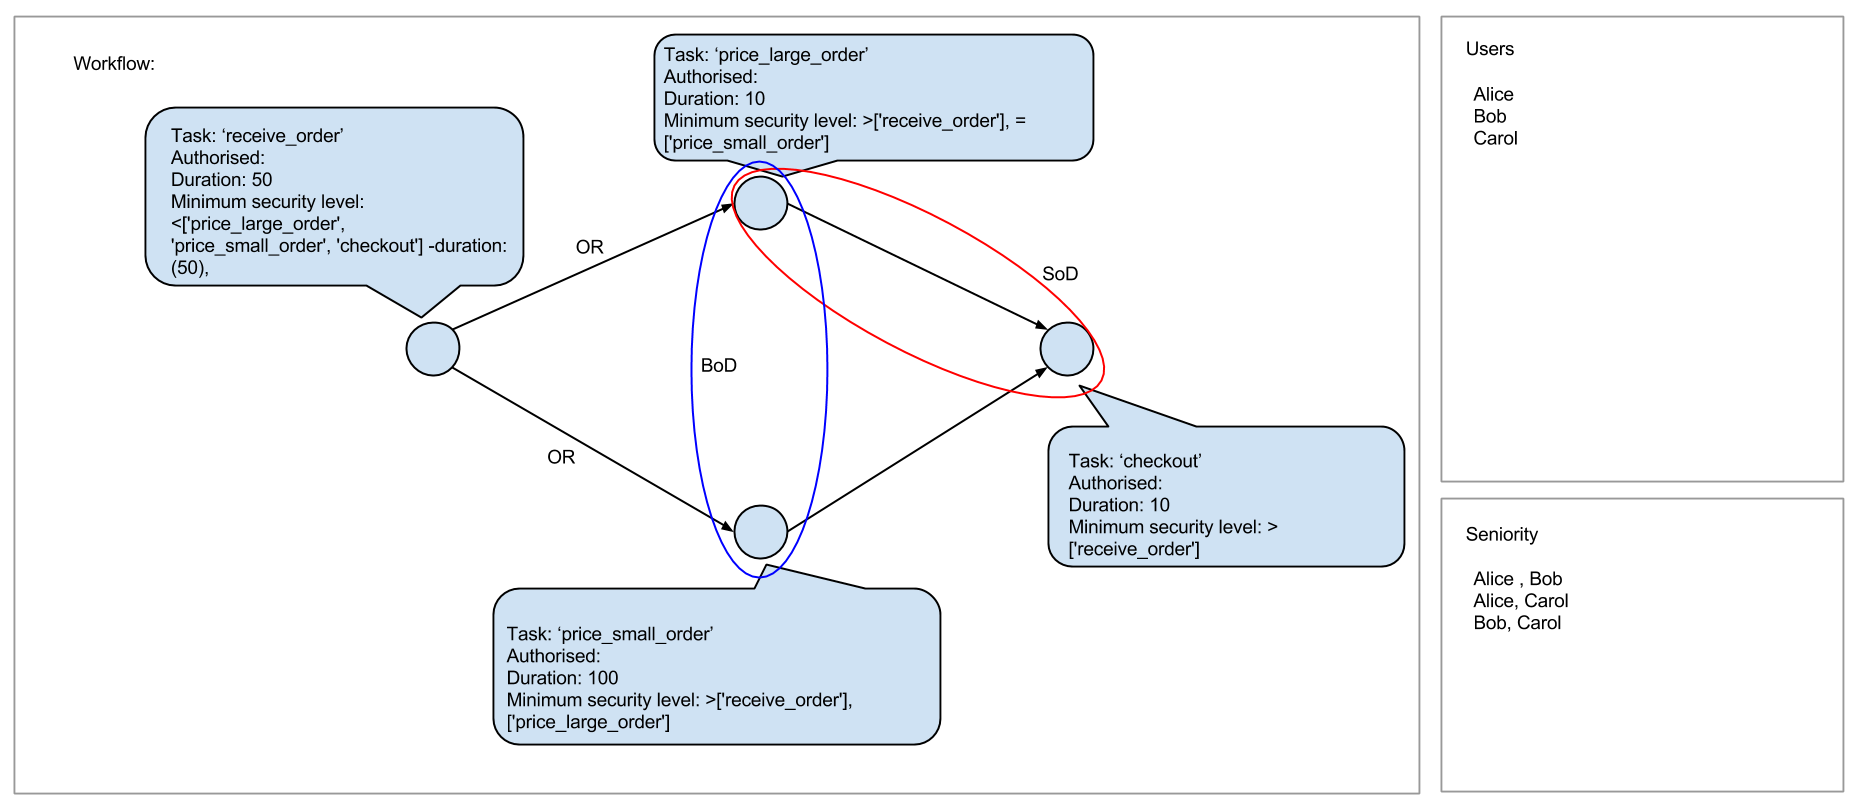
\includegraphics[scale=0.35, angle=90,origin=c]{ui.png}
\caption{Application UI}
\label{fig:Application UI}
\end{figure}

\section{Future Work for a Product}
As the project stands, it is not ready to be used in industry as there are many other constraints that we have not explored that are currently conveyed in business processes. This application may have been aimed at organisations with moderately sized workflows. For example, we have defined a seniority rule where the user must input all the different users and who is senior from each other. Instead, what we could have done is have roles express levels of seniority such as ``associate'' and ``manager'' implemented as \texttt{associate(User)} and \texttt{manager(User)} receptively and then have underlying rules which roles and therefore users are senior to each other. This would save a lot of time for the user when using this application.\\

Hopefully in a few years time and if work continued on this application to build more constraints, it could be used as a workflow constraint solver. \\

\chapter{Appendix A: How to Use and Result Returned}

\bibliography{Master}

\end{document}
